% Una plantilla para LA-CoNGA
% Preguntas: JAL (trabajo en proceso)
% Hecha modificando la siguiente plantilla:
%%%%%%%%%%%%%%%%%%%%%%%%%%%%%%%%%%%%%%%%%
% Beamer Presentation
% LaTeX Template
% Version 1.0 (10/11/12)
%
% This template has been downloaded from:
% http://www.LaTeXTemplates.com
%
% License:
% CC BY-NC-SA 3.0 (http://creativecommons.org/licenses/by-nc-sa/3.0/)
%
%%%%%%%%%%%%%%%%%%%%%%%%%%%%%%%%%%%%%%%%%

%Detallitos:
% https://tex.stackexchange.com/questions/54667/how-can-i-clear-the-color-of-title-in-titlepage
% https://tex.stackexchange.com/questions/178800/creating-sections-each-with-title-pages-in-beamers-slides
% https://cepr.org/sites/default/files/events/1819_Creating%20Presentations%20for%20Widescreen%20laptops.pdf

%----------------------------------------------------------------------------------------
%	PACKAGES AND THEMES
%----------------------------------------------------------------------------------------

\documentclass[aspectratio=169,show notes]{beamer}

%%%% Esta sección "acomoda" el texto de la lámina de una forma más acorde al diseño del fondo
\makeatletter
\setbeamertemplate{frametitle}{
    \ifbeamercolorempty[bg]{frametitle}{}{\nointerlineskip}%
    \@tempdima=\textwidth%
    \advance\@tempdima by\beamer@leftmargin%
    \advance\@tempdima by\beamer@rightmargin%
    \hspace*{1cm} %%%%%%%%%%%%% For example insert shift to right
    \begin{beamercolorbox}[sep=0.15cm,left,wd=\the\@tempdima]{frametitle}
        \usebeamerfont{frametitle}%
        \vbox{}\vskip-1ex%
        \if@tempswa\else\csname beamer@ftecenter\endcsname\fi%
        \strut\insertframetitle\strut\par%
        {%
            \ifx\insertframesubtitle\@empty%
            \else%
            {\usebeamerfont{framesubtitle}\usebeamercolor[fg]{framesubtitle}\insertframesubtitle\strut\par}%
            \fi
        }%
        \vskip-1ex%
        \if@tempswa\else\vskip-.3cm\fi% set inside beamercolorbox... evil here...
    \end{beamercolorbox}%
}
\makeatother

%%%%%%%%%%%
%%% Esta sección crea una lámina automática de inicio de sección
%%%%%%%%%%%
\AtBeginSection[]{
  \begin{frame}
  \vfill
  \centering
  \begin{beamercolorbox}[sep=8pt,center,shadow=true,rounded=true]{title}
    \usebeamerfont{title}\insertsectionhead\par%
  \end{beamercolorbox}
  \vfill
  \end{frame}
}

\mode<presentation> {

\usetheme{default}
\setbeamertemplate{footline}[frame number]
}

\usepackage{graphicx} % Allows including images
\usepackage{booktabs} % Allows the use of \toprule, \midrule and \bottomrule in tables
\usepackage[utf8]{inputenc}
\usepackage[spanish]{babel}

\usepackage[sfdefault]{roboto}  %% Option 'sfdefault' only if the base font of the document is to be sans serif
\usepackage[T1]{fontenc}

\usefonttheme[onlymath]{serif}

\usepackage{fancyvrb}
\usepackage{cprotect}

\usepackage{hyperref}
%\hypersetup{
%    colorlinks=true,
%    linkcolor=blue,
%    filecolor=magenta,      
%    urlcolor=cyan,
%    }

%Colores paleta manual de marca
\definecolor{LCblueInst}{RGB}{50, 50, 123}
\definecolor{LCredInst}{RGB}{237, 28, 36}
\definecolor{LCblueSec1}{RGB}{21, 9, 88}
\definecolor{LCblueSec2}{RGB}{191, 193, 215}
\definecolor{LCblueSec3}{RGB}{247, 248, 249}

%Colores aproximados a los usados en el logo
\definecolor{logoyellow}{RGB}{245, 226, 0}
\definecolor{logobrown}{RGB}{117, 80, 45}
\definecolor{logobrownD}{RGB}{86, 42, 22}

\usepackage{tikz}
\usetikzlibrary{arrows,positioning} 
\tikzset{
    %Define standard arrow tip
    >=stealth',
    %Define style for boxes
    punkt/.style={
           rectangle,
           rounded corners,
           draw=logobrown, very thick,
           text width=4.5em,
           minimum height=2em,
           text centered},
    % Define arrow style
    pil/.style={
           ->,
           draw=logobrown,thick,
           shorten <=2pt,
           shorten >=2pt,}
}
\tikzstyle{resumen} = [rectangle, draw=LCredInst, very thick, fill=LCblueSec2, 
    text width=3.7cm, text justified, rounded corners, minimum height=2cm]
\tikzstyle{socio} = [rectangle,  draw=logobrown, very thick, fill=logoyellow, 
    text width=5.5em, text centered, rounded corners, minimum height=2em]
%
\def\circledarrow#1#2#3{ % #1 Style, #2 Center, #3 Radius
\draw[#1,->] (#2) +(60:#3) arc(60:-230:#3);
}

%----------------------------------------------------------------------------------------
%	TITLE PAGE
%----------------------------------------------------------------------------------------

\title{LA-CoNGA-physics: Latin American alliance for Capacity buildiNG in Advanced physics}

%\title[Short title]{LA-CoNGA} % The short title appears at the bottom of every slide, the full title is only on the title page

\author{José Antonio López {\it (en nombre de LA-CoNGA-physics)}} % Your name
\institute[UCV LA-CoNGA-physics] % Your institution as it will appear on the bottom of every slide, may be shorthand to save space
{
Universidad Central de Venezuela \\ % Your institution for the title page
\textit{jose.lopez@ciens.ucv.ve} % Your email address
}
\date{20 de marzo de 2021} % Date, can be changed to a custom date

%%%%%%%%%%%%%%%%%%%
%% Colores para lámina de título fondo azul
%%%%%%%%%%%%%%%%%%%
\setbeamercolor*{title}{fg=white}
\setbeamercolor*{author}{fg=white}
\setbeamercolor*{institute}{fg=white}
\setbeamercolor*{date}{fg=white}
\setbeamercolor*{frametitle}{fg=white}

\begin{document}
%%%%%%%%%%%%%%%%%%%%%%%%%
%%%%%%% Hay tres opciones de fondo para el titulo
%%%%%%%%%%%%%%%%%%%%%%%%%
\usebackgroundtemplate{
\includegraphics[width=\paperwidth]{plantillas-laconga_1.jpg}}
%\usebackgroundtemplate{\includegraphics[width=\paperwidth]{plantillas-laconga_2.jpg}}
%\usebackgroundtemplate{\includegraphics[width=\paperwidth]{plantillas-laconga_3.jpg}}
\begin{frame}
\titlepage % Print the title page as the first slide
\end{frame}
%%%%%%%%%%%%%%%%%%%%%%%%%%%
%%%%% Cambio el fondo de la lámina según necesidad. El cambio permanece
%%%%%%%%%%%%%%%%%%%%%%%%%%%
%%%%%%
%Los fondos 5, 6, 7 y 8 son creados para texto
% 5 y 6 tienen gradiente de color (no son mis favoritos)
% 5 y 7 tienen pie de pagina (no me funciona en este theme)
\usebackgroundtemplate{
\includegraphics[width=\paperwidth]{plantillas-laconga_8.jpg}}
\begin{frame}
\frametitle{Contenido} % Table of contents slide, comment this block out to remove it
\tableofcontents % Throughout your presentation, if you choose to use \section{} and \subsection{} commands, these will automatically be printed on this slide as an overview of your presentation
\end{frame}

%----------------------------------------------------------------------------------------
%	PRESENTATION SLIDES
%----------------------------------------------------------------------------------------

%------------------------------------------------

%%%%%%%%%%%%%%%%%%%%%%%%%%%%%%%%%%%%%%%%%%%
% cada sección tiene una lámina intro automática
% antes de iniciar una sección uso el fondo 4
% luego de enunciar la sección, regreso al fondo 8
%%%%%%%%%%%%%%%%%%%%%%%%%%%%%%%%%%%%%%%%%%%
\usebackgroundtemplate{
\includegraphics[width=\paperwidth]{plantillas-laconga_4.jpg}}
\section{¿Qué es LA-CoNGA-physics?} % Sections can be created in order to organize your presentation into discrete blocks, all sections and subsections are automatically printed in the table of contents as an overview of the talk
\usebackgroundtemplate{
\includegraphics[width=\paperwidth]{plantillas-laconga_8.jpg}}
%------------------------------------------------

\begin{frame}[fragile]
\frametitle{LA-CoNGA es}
\begin{columns}[c] % The "c" option specifies centered vertical alignment while the "t" option is used for top vertical alignment

\column{.54\textwidth}
\begin{itemize}
\item LA-CoNGA-physics: {\bf L}atin {\bf A}merican alliance for {\bf C}apacity buildi{\bf NG} in {\bf A}dvanced physics.
\item LA-CoNGA physics {\bf \color{LCredInst} es un proyecto de Capacity Building} financiado por {\bf \color{LCblueInst} Erasmus+ Programme Capacity-Building projects in the field of Higher Education (E+CBHE)}.
\item Duración: 3 años.
\item Fecha de inicio: Enero 2020
\end{itemize}


\column{.42\textwidth} % Right column and width
\begin{center}

\includegraphics[scale=0.07]{imagenes/imagotipo-vertical-RGB-grande.png}
\end{center}

\end{columns}
\end{frame}

\begin{frame}[fragile]
\frametitle{Contexto: Sociedad del conocimiento}
\begin{columns}[c] % The "c" option specifies centered vertical alignment while the "t" option is used for top vertical alignment

\column{.38\textwidth}
En la transición a la {\bf \color{logobrown}sociedad del conocimiento} hemos encontrado: 
\begin{itemize}
\item De la sociedad {\bf \color{logoyellow}industrial} a la informacional
\item Economía {\bf \color{LCblueInst}centrada} en conocimiento
\item El conocimiento {\bf \color{LCredInst}es insumo y producto}
\item Producción {\bf \color{LCblueSec1}temprana} de conocimiento
\item Economía {\bf \color{logobrownD}global} interrelacionada
\end{itemize}


\column{.58\textwidth} % Right column and width
\begin{center}

\includegraphics[scale=0.28]{imagenes/socIndustrial.png}
\end{center}

\begin{center}
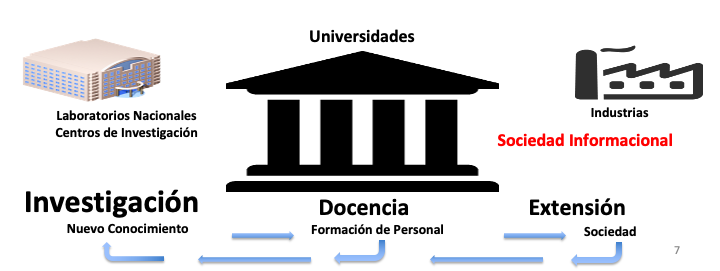
\includegraphics[scale=0.28]{imagenes/socConocimiento.png}
\end{center}
\end{columns}

\end{frame}

\begin{frame}[fragile]
\frametitle{Contexto: la producción del conocimiento}
\begin{columns}[c] % The "c" option specifies centered vertical alignment while the "t" option is used for top vertical alignment

\column{.38\textwidth}
La producción de conocimiento se caracteriza por ser: 
\begin{itemize}
\item Colaborativa
\item Transdisciplinar
\item Global
\item De libre acceso
\item Centrada en grandes volúmenes de datos
\end{itemize}


\column{.58\textwidth} % Right column and width
\begin{center}
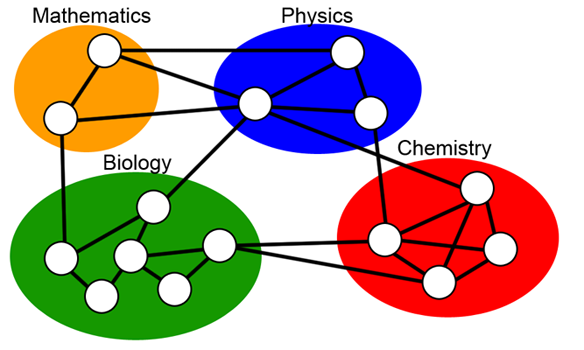
\includegraphics[scale=0.18]{imagenes/Network-of-Scientists3.png}
\end{center}

\begin{center}
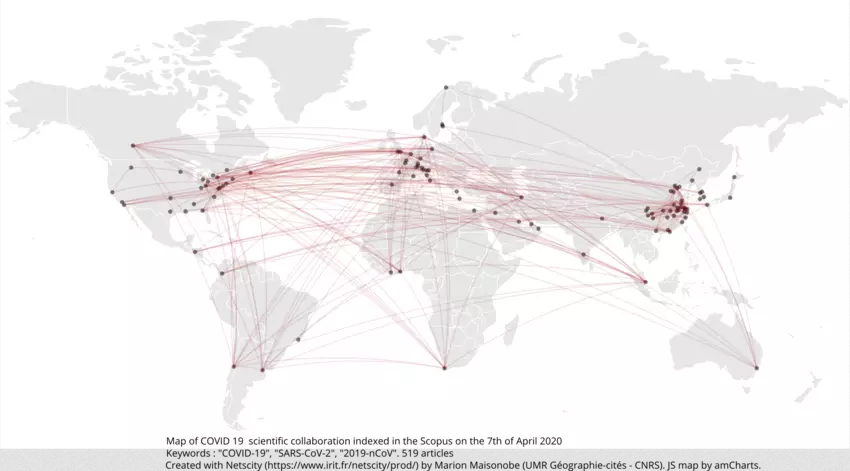
\includegraphics[scale=0.18]{imagenes/covid19_collab.png}
\end{center}
\end{columns}
\vspace{0.25cm}

{\tiny \href{https://blogs.cornell.edu/info2040/2011/09/26/scientific-collaboration-throughout-history-knowledge-networks-with-weak-local-bridges/}{\color{cyan} https://blogs.cornell.edu/info2040/2011/09/26/scientific-collaboration-throughout-history-knowledge-networks-with-weak-local-bridges/}}

{\tiny \href{https://www.weforum.org/agenda/2020/05/global-science-collaboration-open-source-covid-19/}{\color{cyan} https://www.weforum.org/agenda/2020/05/global-science-collaboration-open-source-covid-19/}}

\end{frame}

\note{Everything you want}

\begin{frame}[fragile]
\frametitle{Colaboración científica y educación a escala global}
 
\begin{itemize}
\item En la era de la información, la {\bf \color{LCblueInst}ciencia y la educación} superior se han convertido muy rápidamente en actividades {\bf \color{LCredInst}colaborativas, multidisciplinarias y distribuidas globalmente}.

\item El vínculo universidades-investigación-sociedad es más fuerte: generación de conocimiento, su aplicación y transferencia ocurren en el mismo contexto físico y social. 

\item Las {\bf \color{logoyellow}redes virtuales de investigación y aprendizaje} (Virtual Research and Learning Networks, {\bf \color{logobrownD}VRLN}) juegan un rol fundamental.

\vspace{0.5cm}

{\bf VRLN:} {\bf \color{logobrownD}Infraestructuras de información y comunicación} que combinan {\bf \color{LCredInst}datos}, herramientas de {\bf \color{LCblueInst}software y centros de investigación} para desarrollar plenamente las actividades de docencia e investigación.
\end{itemize}

\end{frame}

\begin{frame}[fragile]
\frametitle{Objetivos de una VRLN}
\begin{columns}[c] % The "c" option specifies centered vertical alignment while the "t" option is used for top vertical alignment

\column{.58\textwidth}
\begin{itemize}
\item {\bf Accesibilidad:}
Cada institución en una VRLN accede a una {\bf \color{LCredInst}cantidad mayor de recursos} y staff académico.

\item {\bf Modernización:}
Mediante el uso de las TICs y los recursos de educación abierta, conectividad, {\bf \color{LCredInst}adquisición de competencias digitales}, el uso y el desarrollo de nuevos medios de aprendizaje. Todo esto {\bf \color{LCblueInst}basado en las capacidades locales}, logrando apropiación y sostenibilidad de los proyectos.

\item {\bf Internacionalización:}
Entrenamiento de nuevas generaciones dentro de un {\bf \color{logoyellow}ambiente colaborativo internacional}.
Aumentando la diversidad en el área.

\end{itemize}


\column{.38\textwidth} % Right column and width
\begin{center}

\includegraphics[scale=0.18]{imagenes/vrln.png}
\end{center}
\end{columns}
\end{frame}

\iffalse
\begin{frame}[fragile]
\frametitle{Física de Altas Energías, Astropartículas y Cosmología en América Latina}
\begin{columns}[c] % The "c" option specifies centered vertical alignment while the "t" option is used for top vertical alignment

\column{.58\textwidth}
Me gustaría transformar esta lámina para hablar de las fortalezas regionales de ambas filiales y salir del contexto LASF4RI
\begin{itemize}
	\item High energy, cosmology and astroparticle physics (HECAP) community/activities has
undoubtedly grown in Latin America in the last decades
	\item A series of initiatives have contributed to it (non exhaustive list)
	\begin{itemize}
		\item The Pierre Auger observatory in Argentina
		\item HELEN and EPLANET programs
		\item Several other national, bi-national or multinational projects
		\end{itemize}
	\item In terms of human and research resources the HECAP development is nuanced and
variable country-by-country (this impacts the training of the new generations)
	\begin{itemize}
		\item Diversity of interests and skills developed (as we see in this forum!)
		\item A young generation with much potential and eagerness to learn
		\item Together we are stronger
		\end{itemize}
	\item HEP is one of the thematic areas of LA-CoNGA physics (another one is complex systems)
\end{itemize}


\column{.38\textwidth} % Right column and width
\begin{center}

\includegraphics[scale=0.18]{imagenes/vrln.png}
\end{center}
\end{columns}
\end{frame}
\fi

\begin{frame}[fragile]
\frametitle{\underline{Misión}, Visión y Valores}
\begin{columns}[c] % The "c" option specifies centered vertical alignment while the "t" option is used for top vertical alignment

\column{.56\textwidth}
Nuestra {\bf\Large \color{LCredInst} misión} es {\bf \color{LCblueSec1} crear una \underline{Comunidad} Latinoamericana y Europea \underline{de Investigación y Aprendizaje} de Física Avanzada} para desarrollar capacidades, {\bf \color{logoyellow} \underline{apoyando la modernización} del sistema de educación superior} y promoviendo valores de {\bf \color{logobrown} colaboración, educación e investigación abierta en \underline{universidades} y \underline{organismos} de \underline{investigación} de \underline{Colombia}, \underline{Ecuador}, \underline{Perú} y \underline{Venezuela}}.

\column{.40\textwidth} % Right column and width

\begin{center}
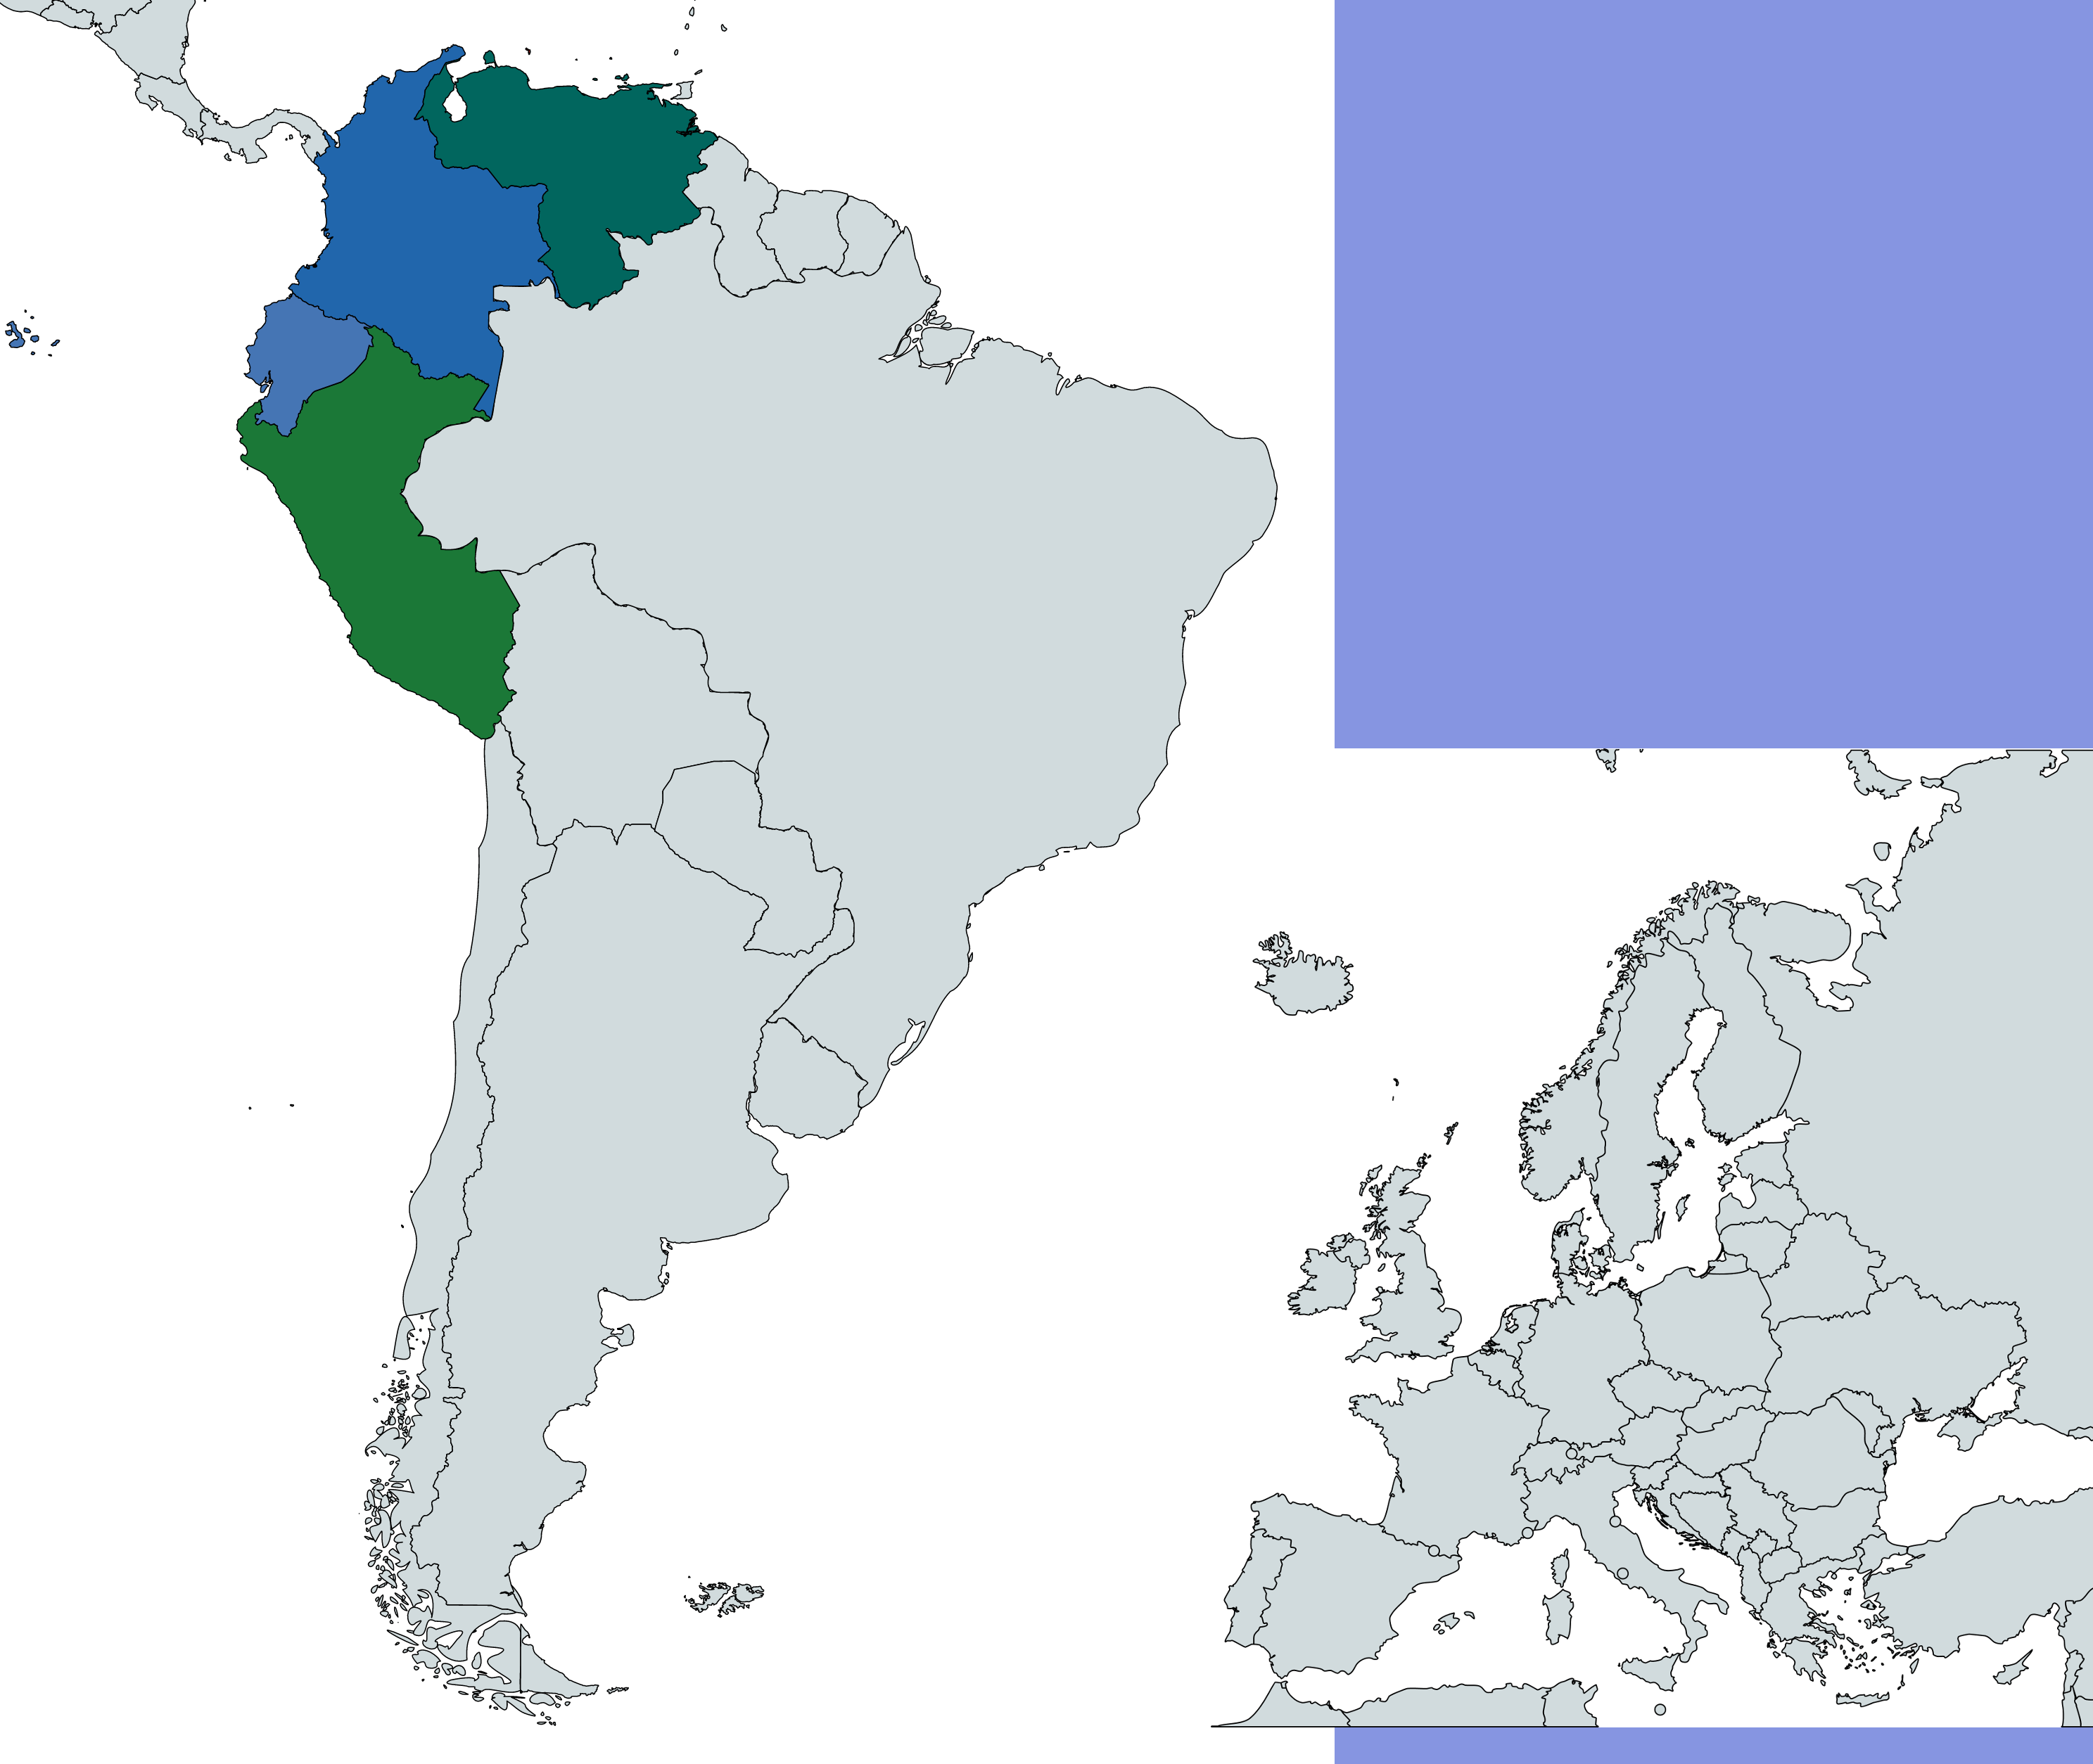
\includegraphics[scale=0.05]{imagenes/mapa_conga_003.png}
\end{center}

\end{columns}



\end{frame}

\begin{frame}[fragile]
\frametitle{Misión, \underline{Visión} y Valores}
\begin{columns}[c] % The "c" option specifies centered vertical alignment while the "t" option is used for top vertical alignment

\column{.58\textwidth}

En LA-CoNGA-physics {\bf \color{LCblueSec1} construimos y cultivamos una red sostenible, dinámica, interconectada y diversa} de investigadores latinoamericanos y europeos en física avanzada, con {\bf \color{LCblueInst} estrechos lazos con el sector productivo, que lidera el desarrollo de la ciencia y la tecnología en la región}. Juntos contribuimos a la modernización, accesibilidad e internacionalización de los sistemas de educación superiores de la región. {\bf\large \color{LCredInst} Nuestra comunidad es una referencia en el contenido curricular, las metodologías educativas utilizadas, e inspira la creación de otras comunidades similares}.

\column{.38\textwidth} % Right column and width
\begin{itemize}
\item Red
\begin{itemize}
\item Sostenible
\item Dinámica
\item Diversa
\end{itemize}
\item Sectores académico y productivo
\item Innovación curricular 
\end{itemize}


\end{columns}



\end{frame}

\begin{frame}[fragile]
\frametitle{Misión, Visión y \underline{Valores}}
\begin{columns}[c] % The "c" option specifies centered vertical alignment while the "t" option is used for top vertical alignment

\column{.32\textwidth}

\begin{itemize}
\item Excelencia
\item Apertura
\item Transparencia
\item Colaboración
\item Respeto
\end{itemize}

\column{.66\textwidth} % Right column and width
Estamos {\bf \color{LCredInst}comprometidos con la \underline{excelencia}, la \underline{apertura} y la \underline{transparencia}} en nuestras actividades educativas y de investigación. {\bf \color{LCblueInst}\underline{Colaboramos}}. Nos comunicamos con palabras, acciones e imágenes que inspiran grandeza, y evitamos las que puedan incomodar a los demás. Fomentamos las discusiones animadas y constructivas. {\bf \color{LCblueSec1}Nos tratamos unos a otros con \underline{respeto} y consideración}.  Acogemos y asesoramos a los miembros nuevos. Fomentamos las ideas novedosas, el debate constructivo. Apoyamos el diálogo entre la teoría y la práctica, entre la academia y la sociedad. {\bf \color{LCblueSec2}\underline{Valoramos} nuestros \underline{orígenes}, \underline{talentos} y \underline{experiencias diversas}}. Siempre estamos abiertos a sugerencias sobre cómo hacerlo mejor.
\end{columns}

\end{frame}

%------------------------------------------------
%%%%%%%%%%%%%%%%%%%%%%%%%%%%%
%%%% Mosca: sección nueva
%%%% Juego con el cambio de fondo: se pasa al 4 y se regresa al 8
%%%%%%%%%%%%%%%%%%%%%%%%%%%%%
\usebackgroundtemplate{
\includegraphics[width=\paperwidth]{plantillas-laconga_4.jpg}}
\section{¿Quiénes somos?}
\usebackgroundtemplate{
\includegraphics[width=\paperwidth]{plantillas-laconga_8.jpg}}
%------------------------------------------------

\begin{frame}[fragile]
\frametitle{LA-CoNGA somos un consorcio}

\begin{tikzpicture}[node distance=1.25cm, auto,]
 %nodes
 \node[inner sep=0pt] (mapa) at (7.2,-3.2)
    {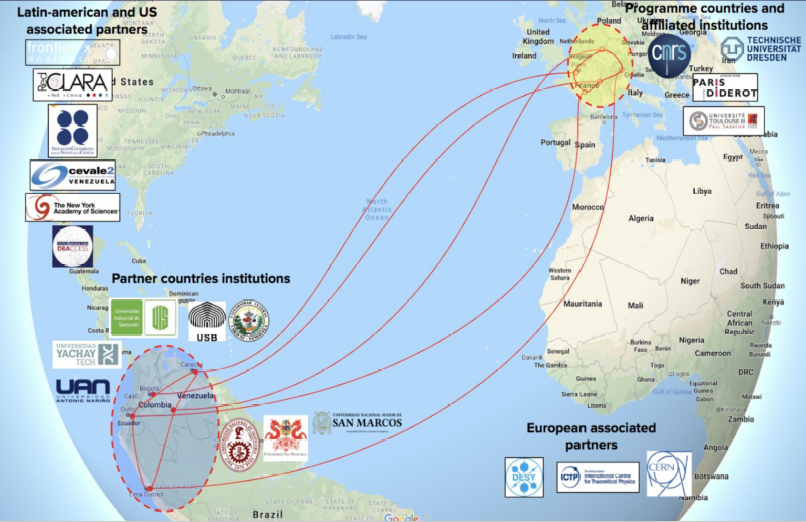
\includegraphics[scale=0.35]{imagenes/mapaColab.png}};
 \node[socio] (academic) at (0,-0.9) {{\small Socios Académicos}};
 \node[below=of academic] (dummy1) {};
 \node[socio, right=of dummy1] (industrial) {\small Socios Industriales}
 	edge[pil,<->,bend right=45] (academic.east);
 \node[below=of dummy1] (dummy2) {};
 \node[below=of dummy2] (dummy) {};
 \node[socio,left=of dummy2] (cientific){\small Socios Científicos}
 	edge[pil,<->,bend left=45] (academic.west)
 	edge[pil,<->,bend right=45] (industrial.south);
 \node[right=of industrial] (dummy3) {};
 \node[right=of dummy3] (dummy4) {};
 %\node[resumen, below=of dummy3] (resumen) {{\bf\color{LCredInst} Resumen}\begin{itemize}
 \node[resumen] (resumen) at (1.5,-5.8) {\small \begin{itemize}
 \item[-] Universidades (11)
 \item[-] Socios científicos e industriales (13)
 \item[-] Total: 24 instituciones.
 \end{itemize}};
 
 \end{tikzpicture}

\end{frame}

\begin{frame}[fragile]
\frametitle{LA-CoNGA somos: Universidades socias LA}
\begin{columns}[c] % The "c" option specifies centered vertical alignment while the "t" option is used for top vertical alignment

\column{.58\textwidth}
\begin{itemize}
	\item Colombia:
	\begin{itemize}
		\item Universidad Antonio Nariño (UAN)
		\item Universidad Industrial de Santander
(UIS) {\bf (coordinadora LA)}.
		\end{itemize}
	\item Ecuador:
	\begin{itemize}
		\item Universidad San Francisco de Quito
(USFQ).
		\item Universidad Yachay Tech (UYT).
		\end{itemize}
	\item Perú:
	\begin{itemize}
		\item Universidad Nacional de Ingeniería
(UNI).
		\item Universidad Nacional Mayor de San
Marcos (UNMSM).
		\end{itemize}
	\item Venezuela:
	\begin{itemize}
		\item Universidad Central de Venezuela
(UCV).
		\item Universidad Simón Bolívar (USB).
		\end{itemize}
\end{itemize}


\column{.38\textwidth} % Right column and width
\begin{center}
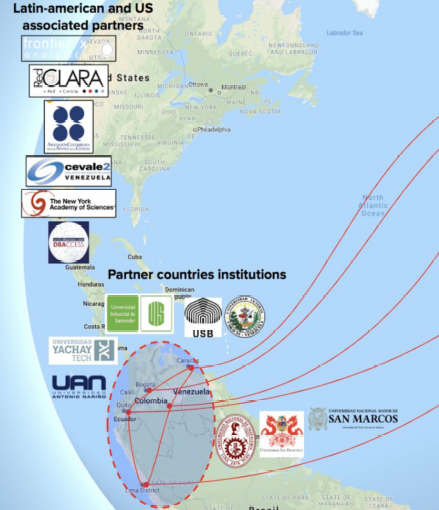
\includegraphics[scale=0.5]{imagenes/mapaColab_1.png}
\end{center}

\end{columns}
\end{frame}


\begin{frame}[fragile]
\frametitle{LA-CoNGA somos: Universidades socias UE}
\begin{columns}[c] % The "c" option specifies centered vertical alignment while the "t" option is used for top vertical alignment

\column{.58\textwidth}
\begin{itemize}
	\item Alemania:
	\begin{itemize}
		\item Technische Universitat Dresden (TUD).
		\end{itemize}
	\item Francia:
	\begin{itemize}
		\item Universitè de Paris (UdP) {\bf (líder)}
		\item Universitè Touluse III Paul Sabatier (UPS)
		\end{itemize}
\end{itemize}

\column{.38\textwidth} % Right column and width
\begin{center}
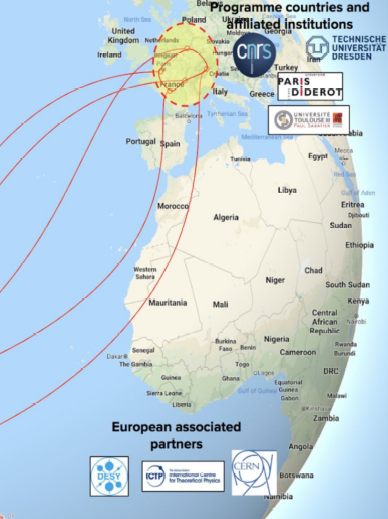
\includegraphics[scale=0.5]{imagenes/mapaColab_2.png}
\end{center}

\end{columns}
\end{frame}

\note{sociosCienInd}

\begin{frame}[fragile]
\frametitle{LA-CoNGA somos: Socios Científicos e Industriales}

\begin{center}

\includegraphics[scale=0.5]{imagenes/sociosCienInd.png}
\end{center}

\end{frame}





%%%%%%%%%%%%%%%%%%%%%%%%%%%%%%%%%%%%%%%%%%%
% cada sección tiene una lámina intro automática
% antes de iniciar una sección uso el fondo 4
% luego de enunciar la sección, regreso al fondo 8
%%%%%%%%%%%%%%%%%%%%%%%%%%%%%%%%%%%%%%%%%%%
\usebackgroundtemplate{
\includegraphics[width=\paperwidth]{plantillas-laconga_4.jpg}}
\section{¿Qué queremos hacer?} % Sections can be created in order to organize your presentation into discrete blocks, all sections and subsections are automatically printed in the table of contents as an overview of the talk
\usebackgroundtemplate{
\includegraphics[width=\paperwidth]{plantillas-laconga_8.jpg}}
%------------------------------------------------

\begin{frame}[fragile]
\frametitle{¿Qué queremos en LA-CoNGA?}
\begin{columns}[c] % The "c" option specifies centered vertical alignment while the "t" option is used for top vertical alignment

\column{.58\textwidth}

\begin{itemize}
	\item {\bf \color{LCredInst} LA-CoNGA physics} desarrolla un programa de {\bf  \color{LCblueInst} especialización en Física avanzada} 
	\item Este programa {\bf  \color{logoyellow} se inserta como especialización en las maestrías de Física} de los socios de LA (8 universidades)
	\item Está inspirado en los {\bf  \color{logobrownD} protocolos de Boloña (60 ECTS)}
	\item Se basa sobre tres pilares
	\begin{itemize}
		\item Ciencia
		\item Datos
		\item Instrumentación
		\end{itemize}
	\item Se guía por los principios de {\bf  \color{LCblueSec1} ciencia y educación abierta}
\end{itemize}


\column{.38\textwidth} % Right column and width
\begin{center}

\includegraphics[scale=0.07]{imagenes/principios.png}
\end{center}

\end{columns}


\end{frame}

\begin{frame}[fragile]
\frametitle{LA-CoNGA quiere estudiar Física de Altas Energías}
\begin{center}
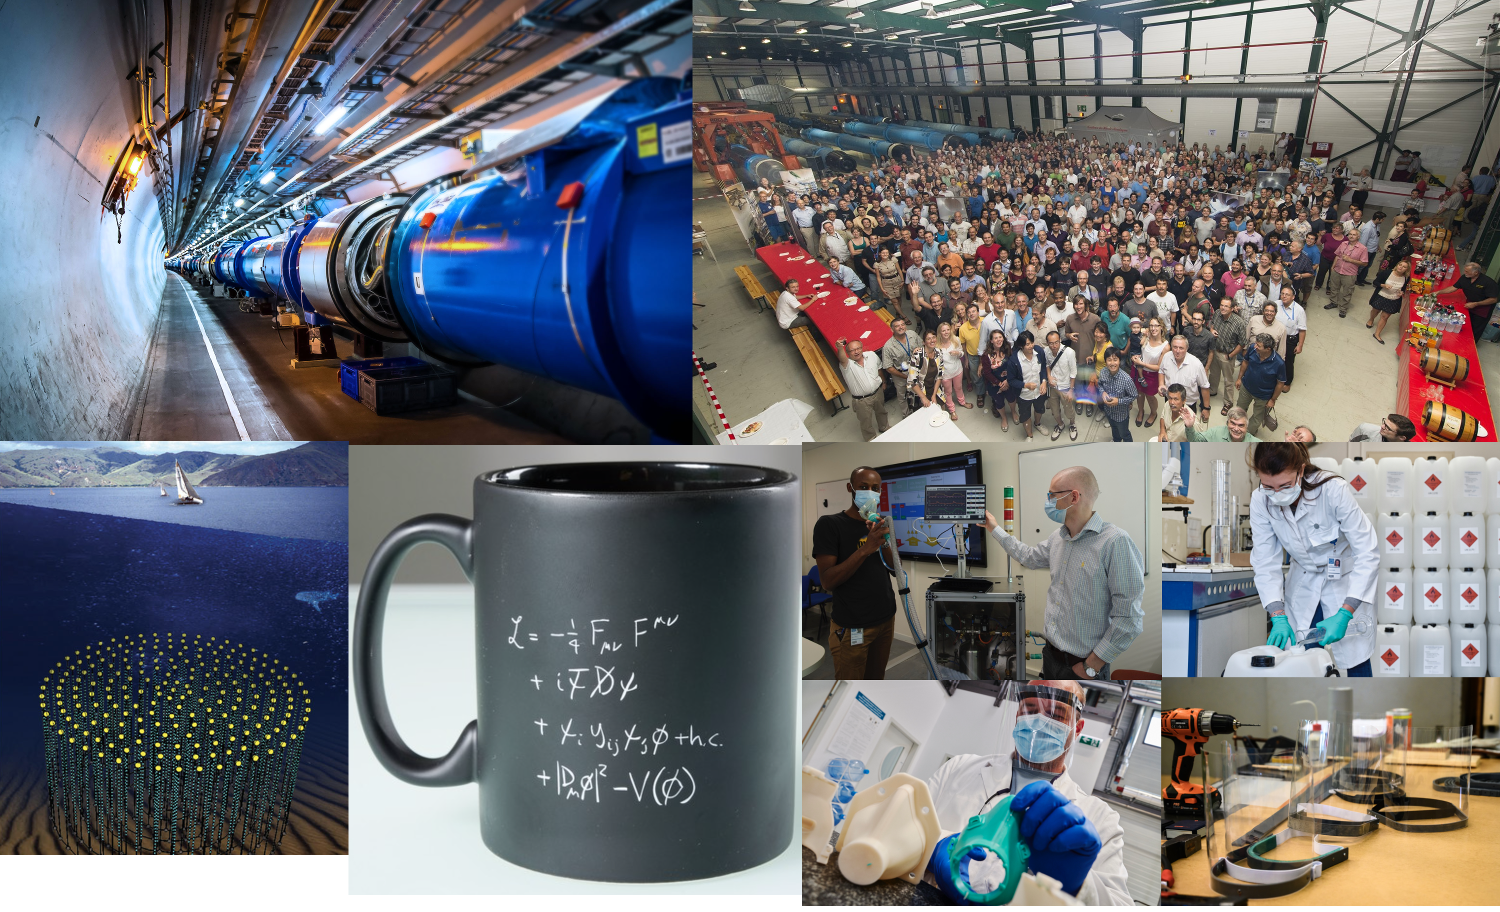
\includegraphics[scale=0.91]{imagenes/fisicaAE.png}
\end{center}
\end{frame}


\begin{frame}[fragile]
\frametitle{LA-CoNGA quiere estudiar Física de los Sistemas Complejos}
\begin{center}
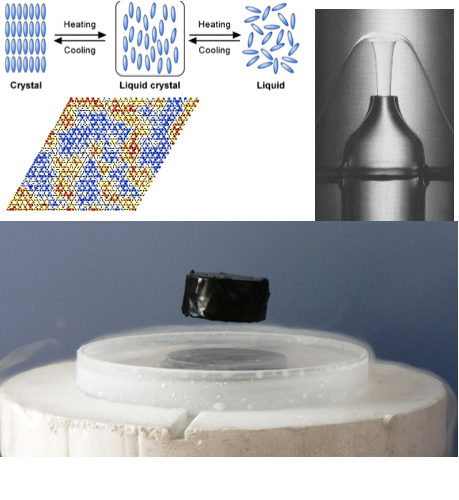
\includegraphics[scale=0.9]{imagenes/fisicaSC1.png}
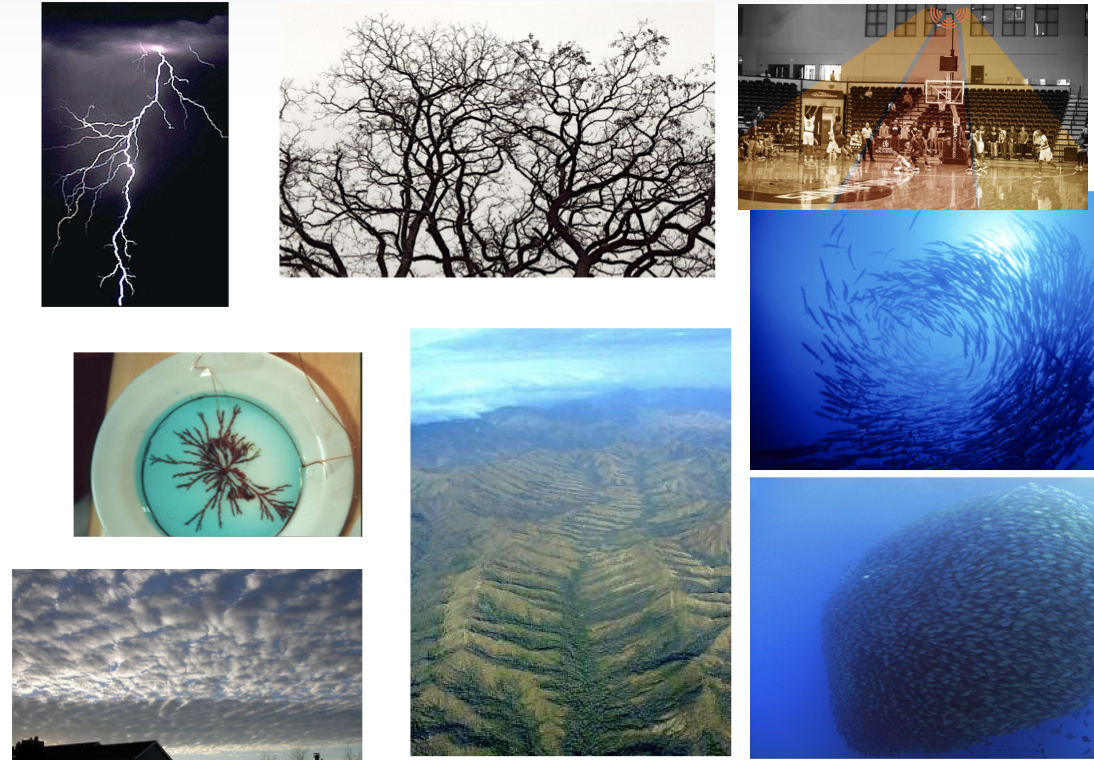
\includegraphics[scale=0.2]{imagenes/fisicaSC2.png}
\end{center}
\end{frame}




%%%%%%%%%%%%%%%%%%%%%%%%%%%%%%%%%%%%%%%%%%%
% cada sección tiene una lámina intro automática
% antes de iniciar una sección uso el fondo 4
% luego de enunciar la sección, regreso al fondo 8
%%%%%%%%%%%%%%%%%%%%%%%%%%%%%%%%%%%%%%%%%%%
\usebackgroundtemplate{
\includegraphics[width=\paperwidth]{plantillas-laconga_4.jpg}}
\section{¿Cómo lo vamos a hacer?} % Sections can be created in order to organize your presentation into discrete blocks, all sections and subsections are automatically printed in the table of contents as an overview of the talk
\usebackgroundtemplate{
\includegraphics[width=\paperwidth]{plantillas-laconga_8.jpg}}
%------------------------------------------------

\begin{frame}[fragile]
\frametitle{LA-CoNGA: Plataforma y Método}
\begin{columns}[c] % The "c" option specifies centered vertical alignment while the "t" option is used for top vertical alignment

\column{.60\textwidth}
\begin{itemize}\small
	\item Plataforma de {\it e-learning} integrada
	\begin{itemize}
		\item Acceso remoto a una red de laboratorios interconectados
		\item Recursos docentes
		\item Repositorios de datos e información
		\item Recursos de comunicación
		\item Computación en la nube
	\end{itemize}
	\item Currículo 
	\begin{itemize}
		\item Distribuido en bloques pequeños
		\item Orientado a la aplicación inmediata de las competencias adquiridas
	\end{itemize}
	\item Buenas prácticas
	\begin{itemize}
		\item Trabajo en colaboración científica
		\item Reproducibilidad científica
	\end{itemize}
	\item Programa de movilidad en LA y UE
	\begin{itemize}
		\item Socios Académicos y Científicos
		\item Socios Industriales
	\end{itemize}	
\end{itemize}
\column{.36\textwidth} % Right column and width
\begin{center}
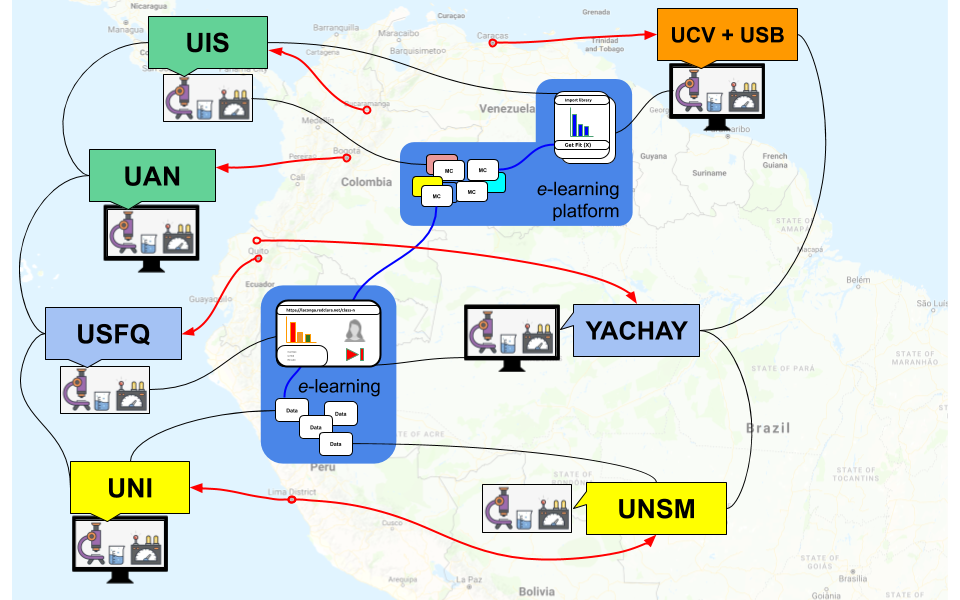
\includegraphics[scale=0.16]{imagenes/labRemotosElearning.png}
\end{center}

\begin{center}
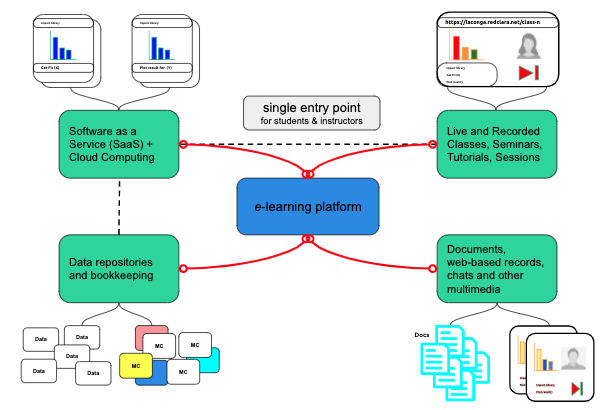
\includegraphics[scale=0.23]{imagenes/Elearning.png}
\end{center}

\end{columns}

\end{frame}

\begin{frame}[fragile]
\frametitle{LA-CoNGA: Plataforma y Método}
\begin{center}

\begin{tikzpicture}[node distance=1.25cm, auto,]
 %nodes
  \node[inner sep=0pt] (logo) at (7.2,-3)
    {
\includegraphics[scale=0.27]{imagenes/isotipo-RGB-pequeno.png}};
  \node (text) at (7.2,-3.1) {};
	\circledarrow{ultra thick, logobrown}{text}{1.7cm};
 \node[inner sep=0pt] (plataforma) at (10.4,-0.5)
    {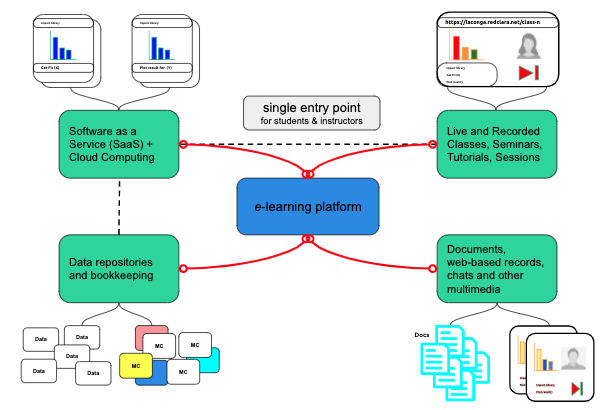
\includegraphics[scale=0.18]{imagenes/Elearning.png}};
 \node[inner sep=0pt] (tools) at (11,-3)
    {
\includegraphics[scale=0.12]{imagenes/logos/logos.png}};
 \node[inner sep=0pt] (clases) at (10,-5.7)
    {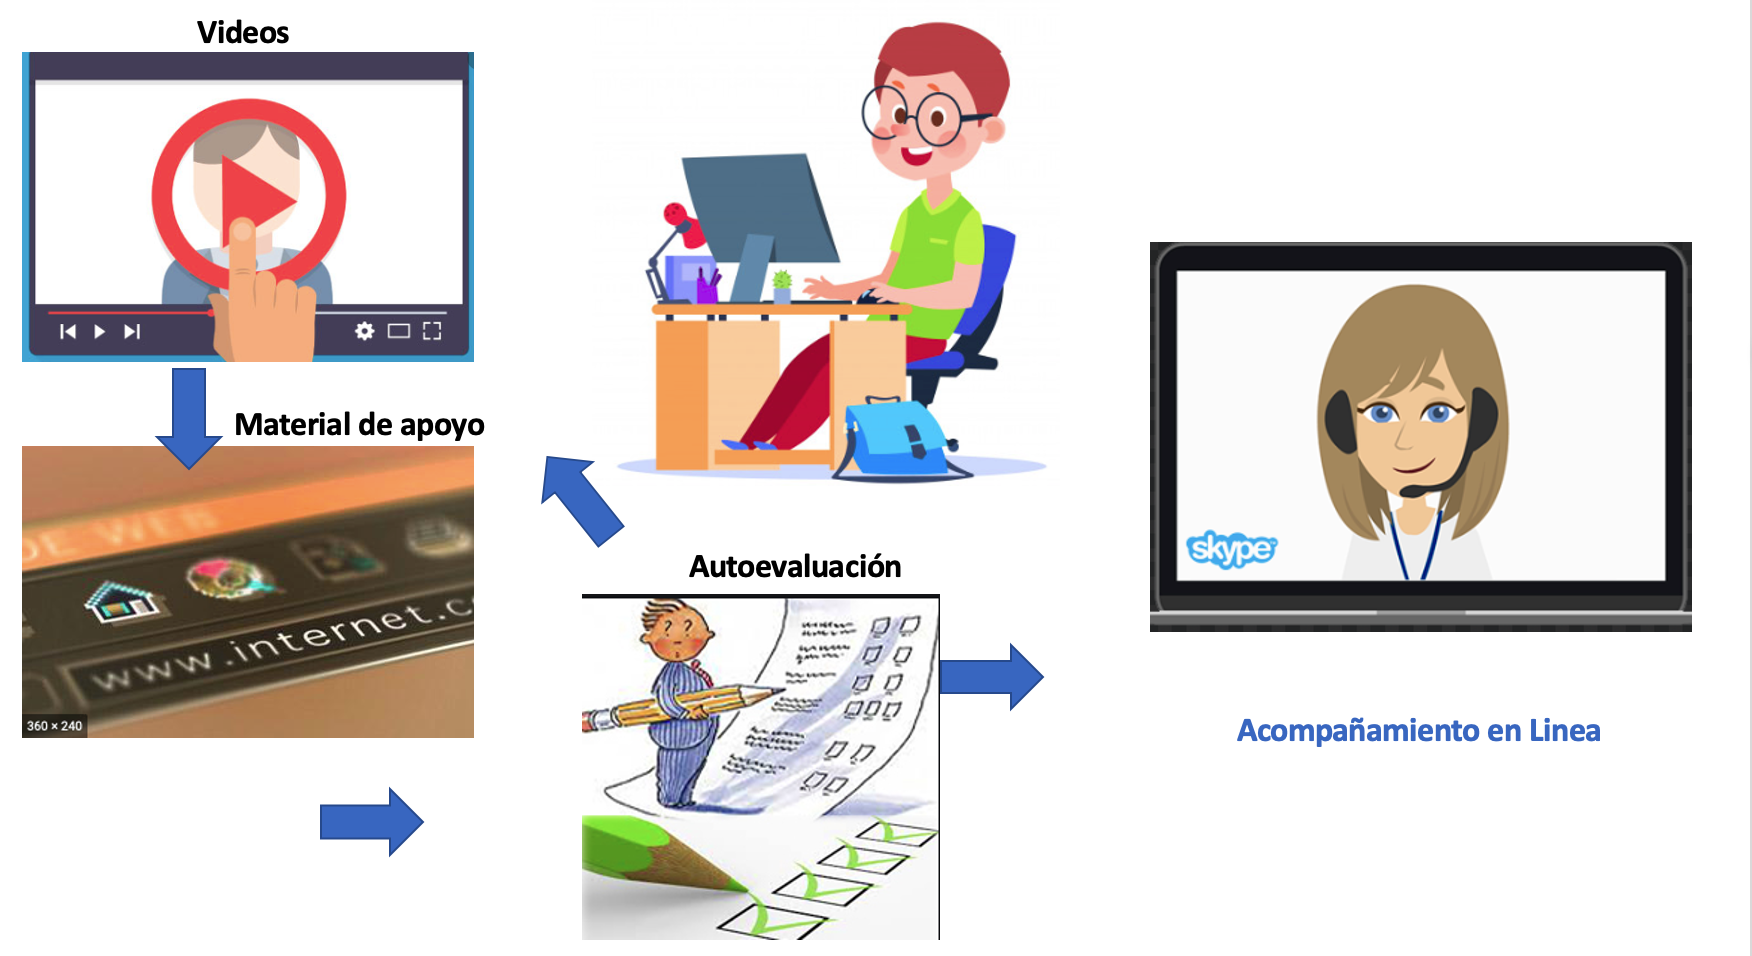
\includegraphics[scale=0.12]{imagenes/clases.png}};
 \node[inner sep=0pt] (bloques) at (5.2,-6)
    {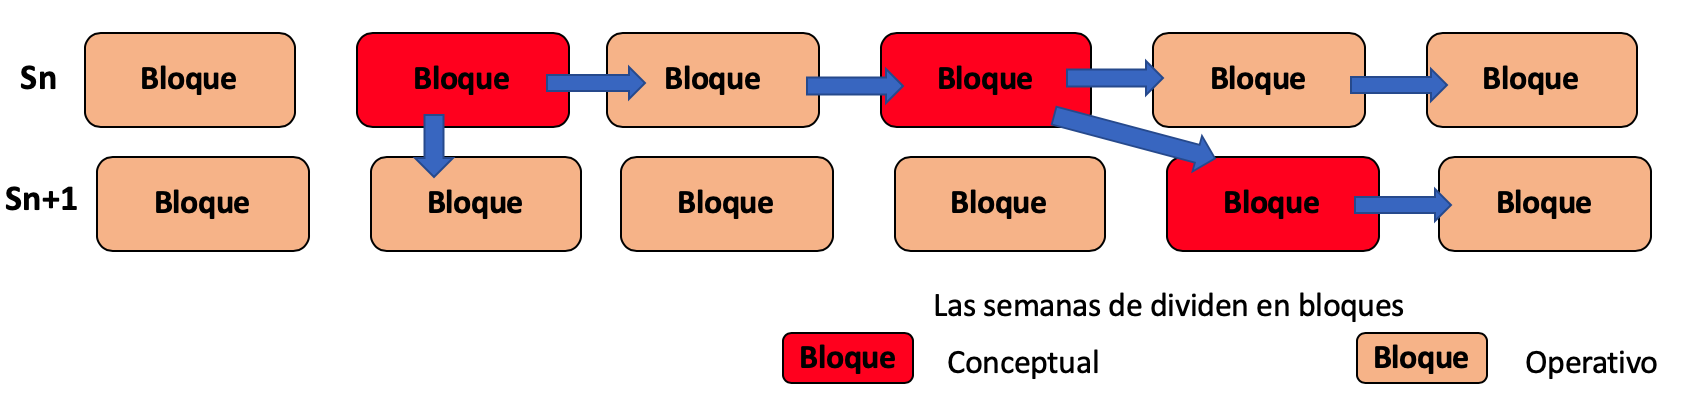
\includegraphics[scale=0.21]{imagenes/bloques.png}};
 \node[inner sep=0pt] (tools) at (3.8,-3.5)
    {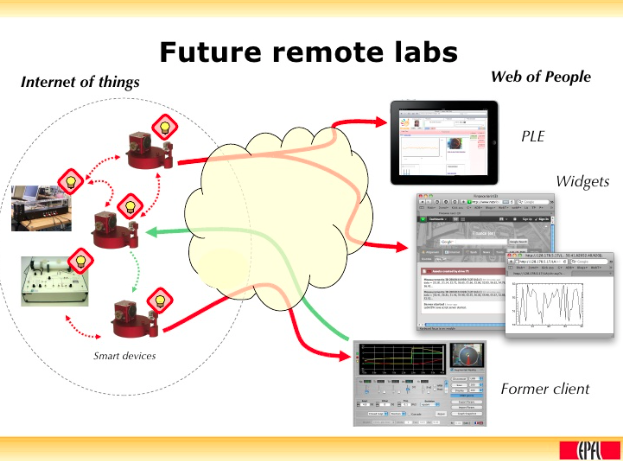
\includegraphics[scale=0.12]{imagenes/remoteLab.png}};
 \node[inner sep=0pt] (reproducibilidad) at (4.2,-0.5)
    {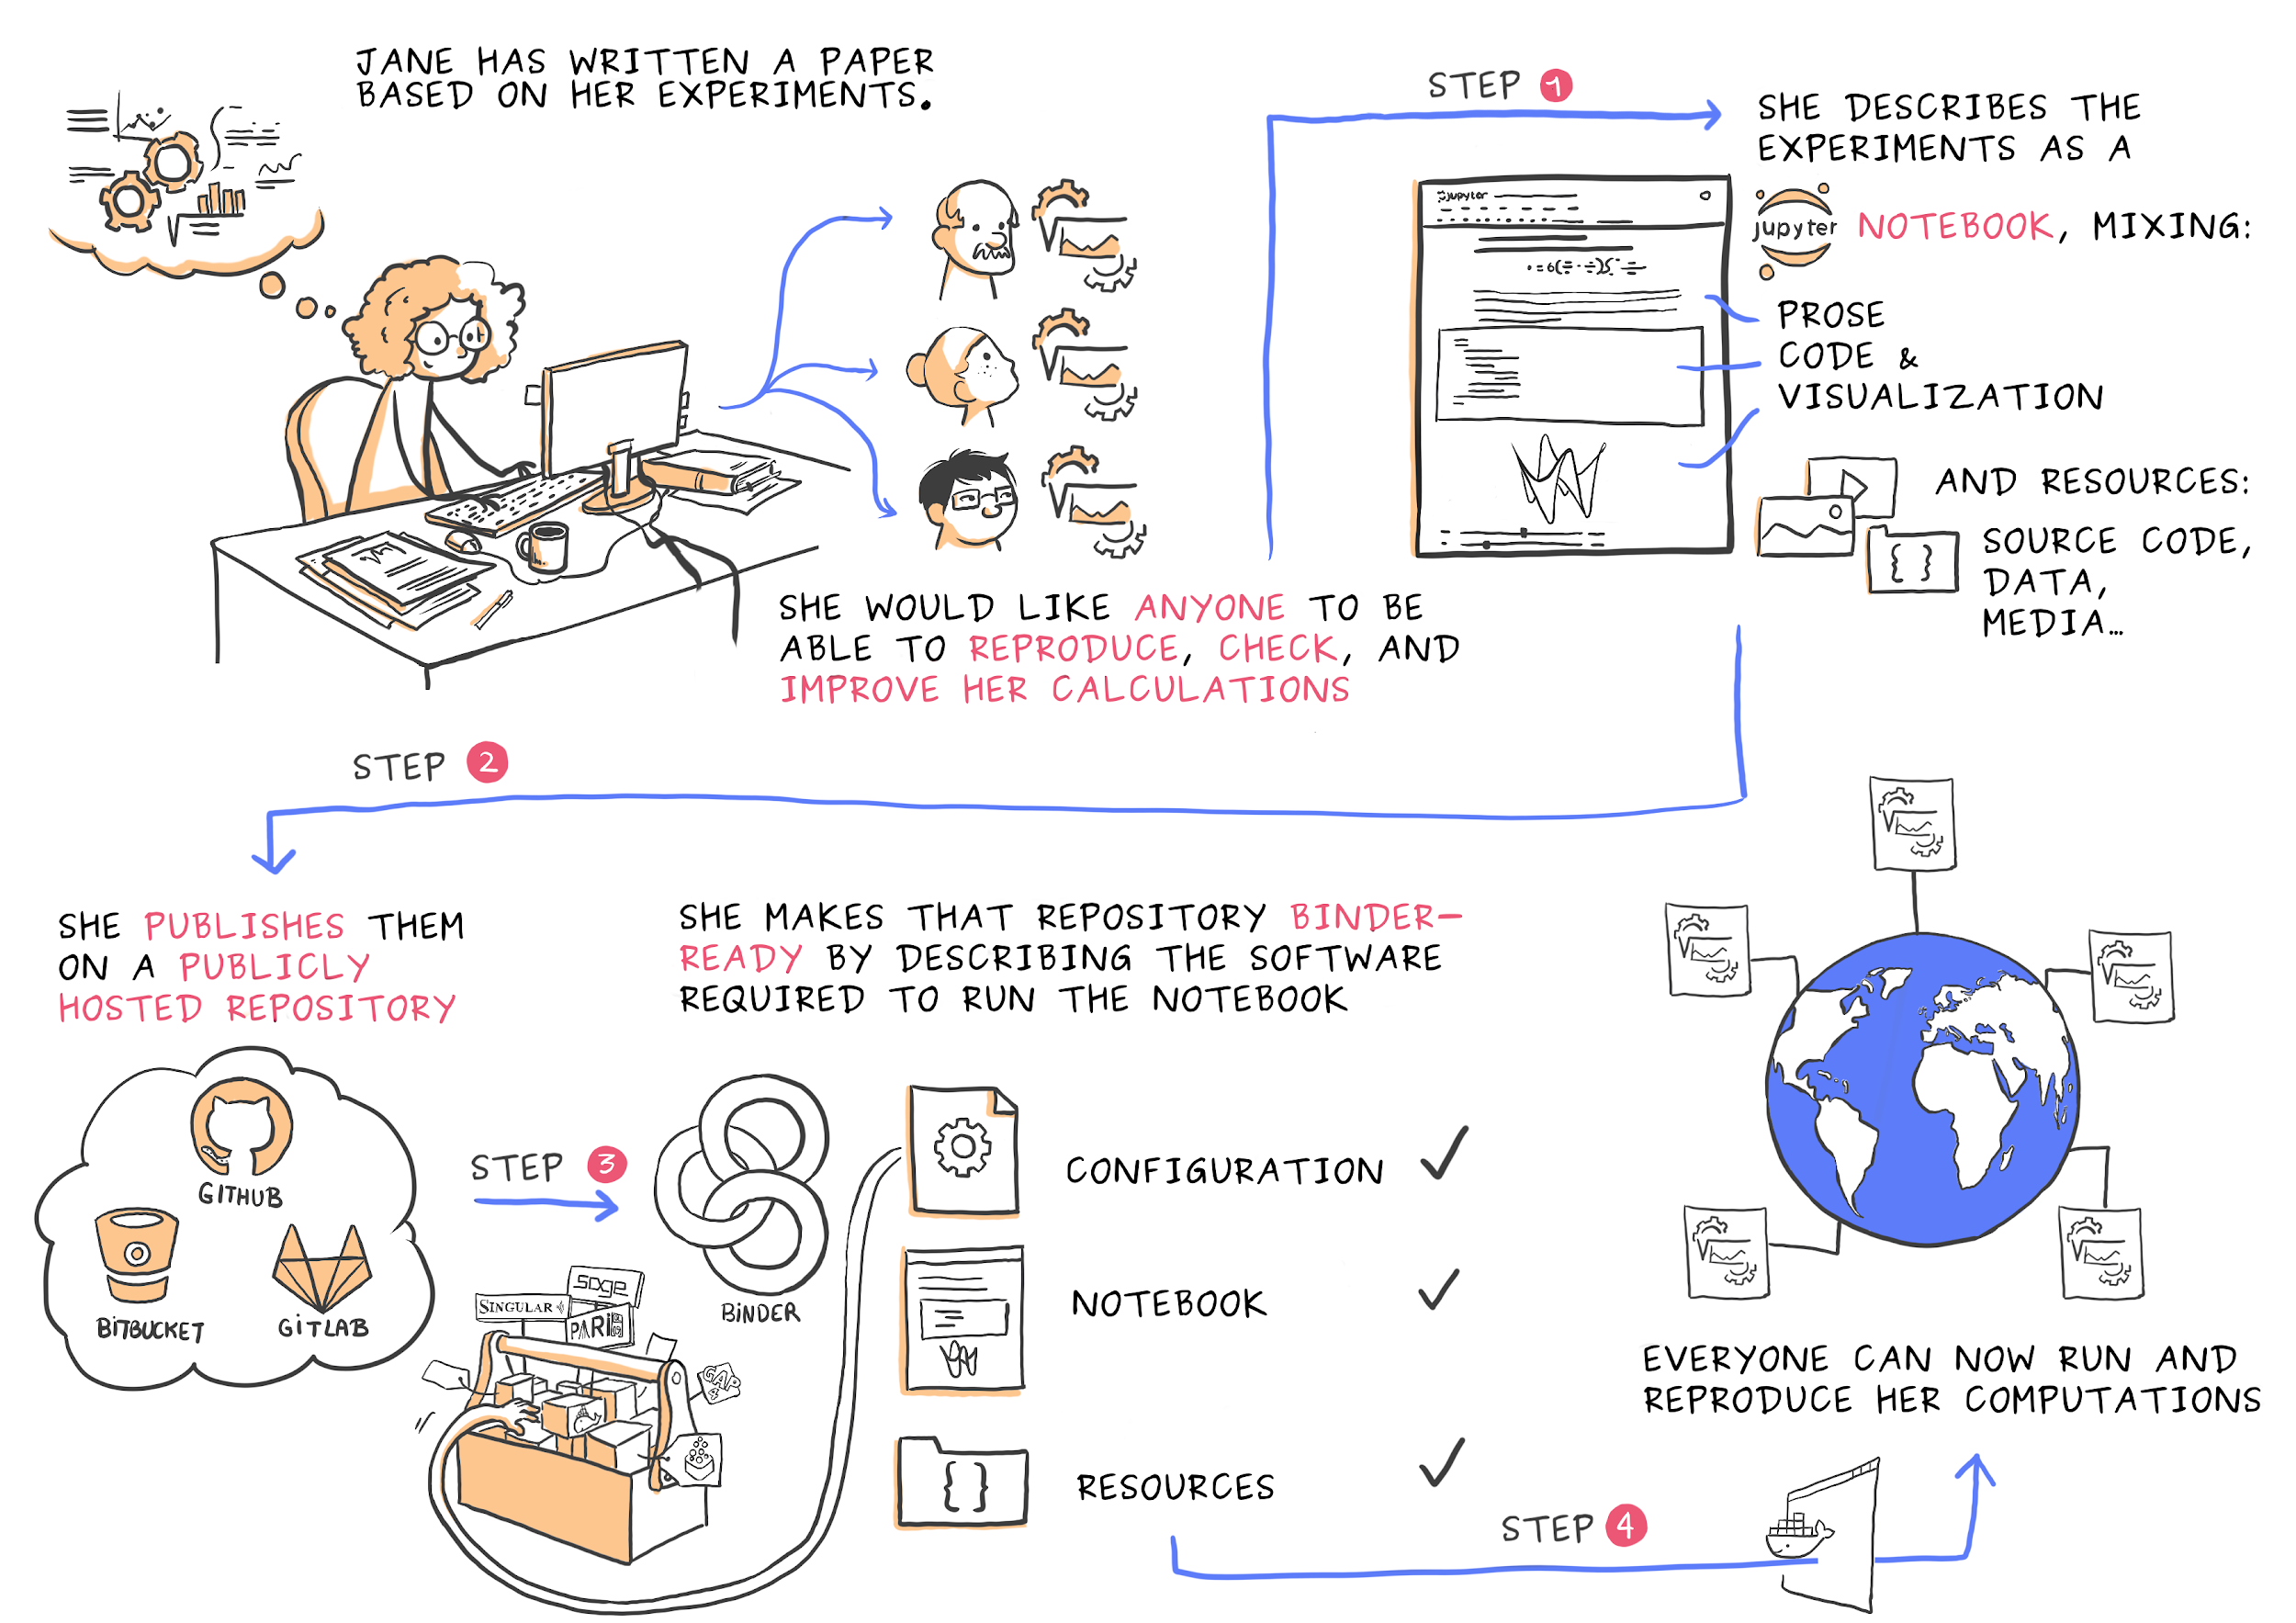
\includegraphics[scale=0.04]{imagenes/reproducibilidad.png}};
 \end{tikzpicture}
 
\end{center}
\end{frame}


\begin{frame}[fragile]
\frametitle{LA-CoNGA: Malla curricular}
\begin{center}
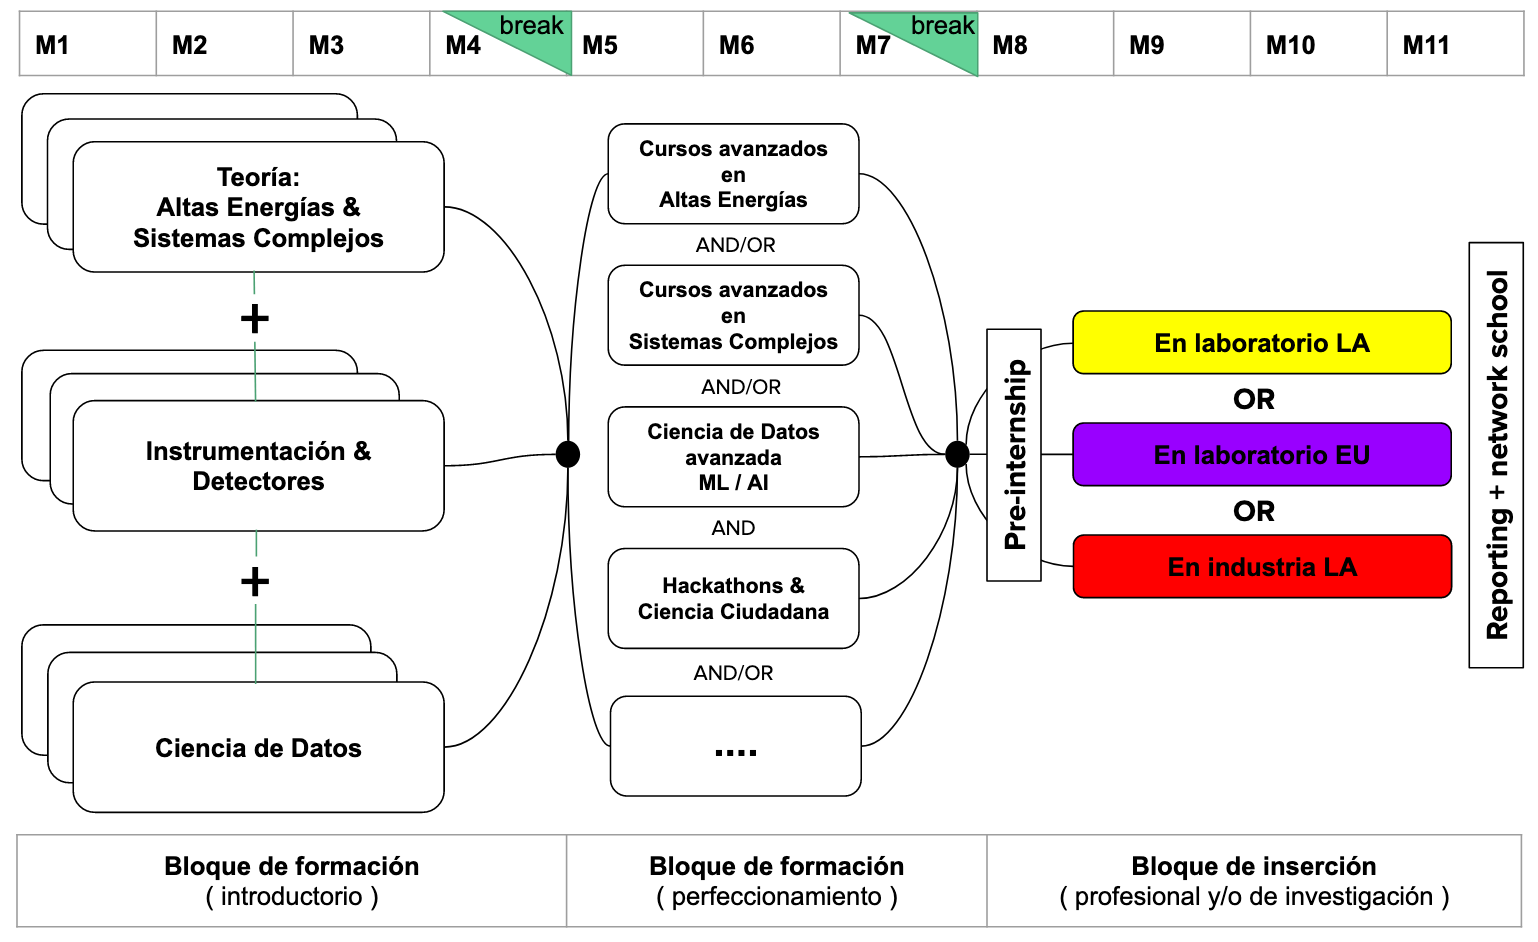
\includegraphics[scale=0.45]{imagenes/MetPlat.png}
\end{center}
\end{frame}

\note{sociosCienInd}







%%%%%%%%%%%%%%%%%%%%%%%%%%%%%%%%%%%%%%%%%%%
% cada sección tiene una lámina intro automática
% antes de iniciar una sección uso el fondo 4
% luego de enunciar la sección, regreso al fondo 8
%%%%%%%%%%%%%%%%%%%%%%%%%%%%%%%%%%%%%%%%%%%
\usebackgroundtemplate{
\includegraphics[width=\paperwidth]{plantillas-laconga_4.jpg}}
\section{LA-CoNGA paso a paso} % Sections can be created in order to organize your presentation into discrete blocks, all sections and subsections are automatically printed in the table of contents as an overview of the talk
\usebackgroundtemplate{
\includegraphics[width=\paperwidth]{plantillas-laconga_8.jpg}}
%------------------------------------------------

\begin{frame}[fragile]
\frametitle{LA-CoNGA ayer: 2020}
\begin{columns}[c] % The "c" option specifies centered vertical alignment while the "t" option is used for top vertical alignment

\column{.54\textwidth}
\begin{itemize}
	\item Enero 2020: comienza la vida del proyecto
	\item ¡COVID-19!
	\begin{itemize}
		\item Nuevo plan de actividades
		\item Aprovechar las características de nuestro proyecto para adaptarnos
		\item Discutirlo, apoyarnos
		\item ¡Cumplir los objetivos!
		\end{itemize}
	\item Conectamos instituciones:
	\begin{itemize}
		\item Convenios interinstitucionales
		\item Inserción de programas en maestrías de las universidades socias
		\item Planificación de equipamiento
		\end{itemize}	
	\end{itemize}
\column{.42\textwidth} % Right column and width
\begin{center}
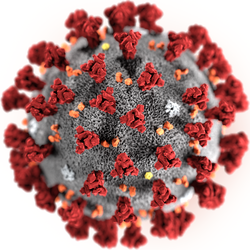
\includegraphics[scale=0.6]{imagenes/SARS-CoV-2_CDC-23312.png}
\end{center}

\end{columns}
\end{frame}

\begin{frame}[fragile]
\frametitle{LA-CoNGA ayer: 2020}
\begin{columns}[c] % The "c" option specifies centered vertical alignment while the "t" option is used for top vertical alignment
\column{.42\textwidth}
\begin{itemize}
	\item Desarrollo de identidad
	\begin{itemize}
		\item Misión, Visión, Valores
		\item RRSS: @lacongaphysics
		\item Manual de imagen
		\end{itemize}
	\item Código de Conducta
	\item Plan de Diversidad
	\item Plan de datos
	\item Proyectos de ciencia ciudadana
	\item Diseño curricular
	\begin{itemize}
		\item Específico semestre A
		\item General para semestre B
		\end{itemize}
	\item Diseño de plataforma
	\begin{itemize}
		\item Selección de herramientas
		\item Desarrollo y pruebas
		\end{itemize}
	\end{itemize}
\column{.54\textwidth} % Right column and width
\begin{center}
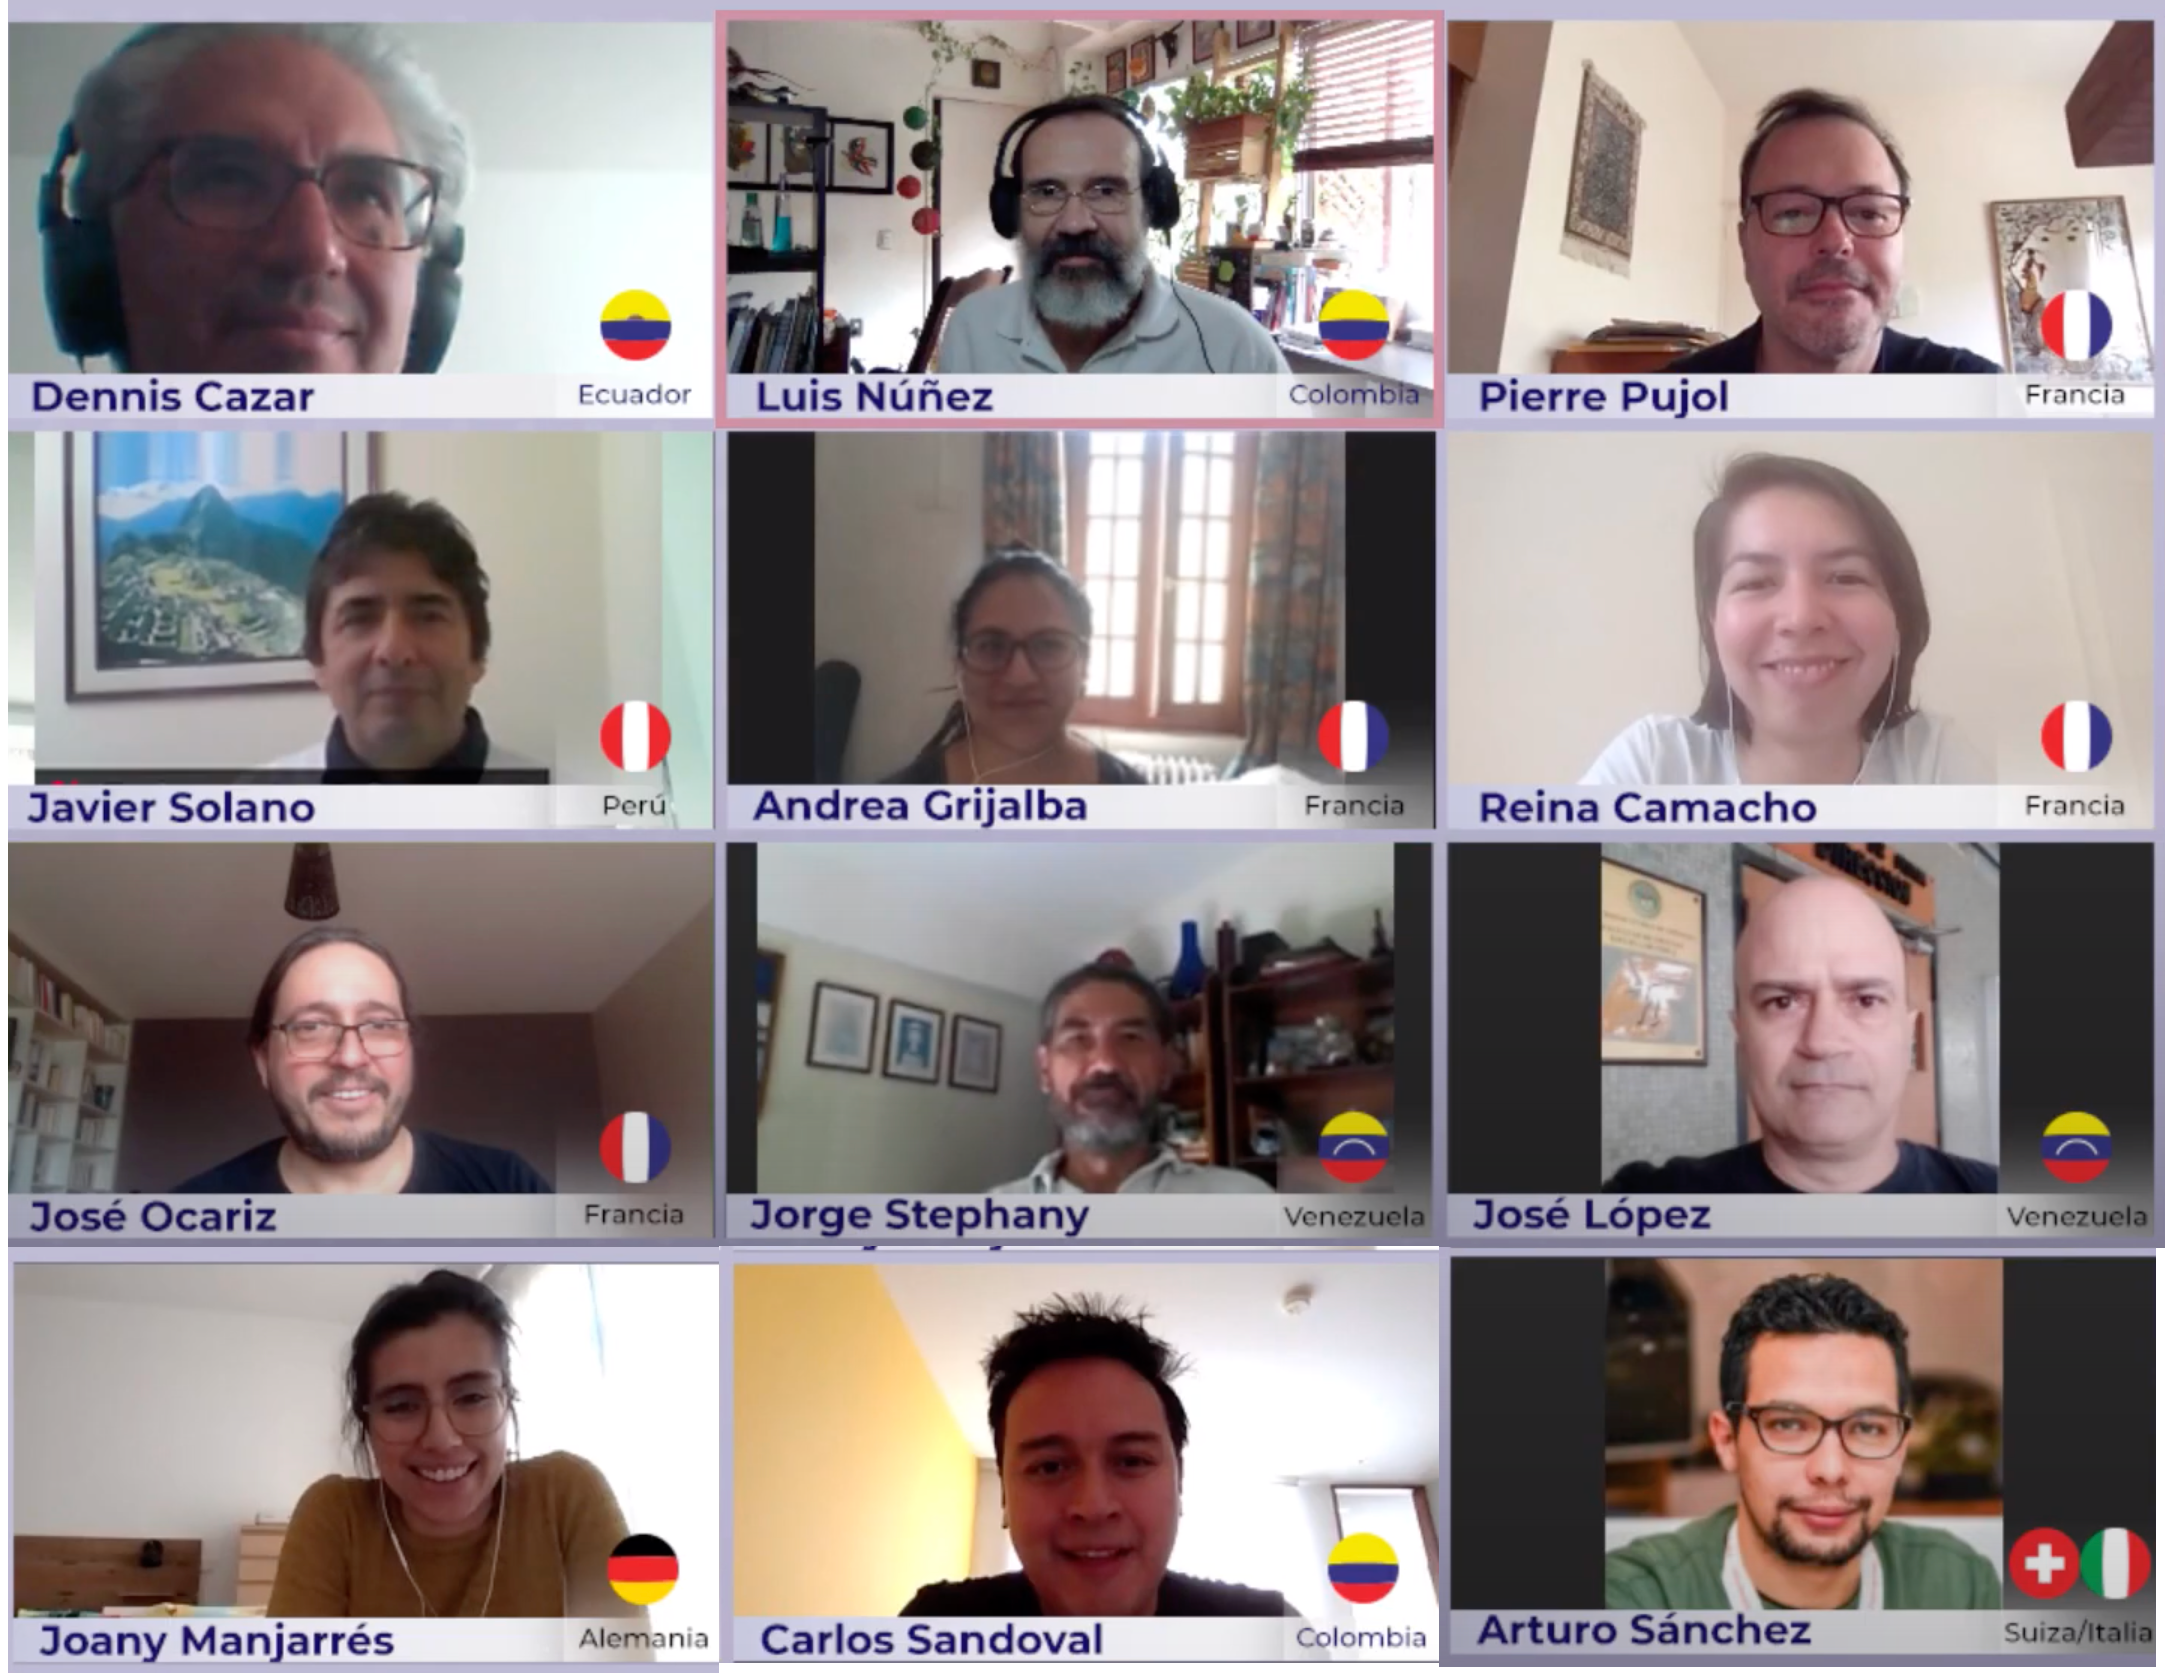
\includegraphics[scale=0.21]{imagenes/TodosLaConga2020_4x3.png}
\vspace{0.05cm}
	
{\tiny Un subgrupo conguero}
\end{center}

\end{columns}
\end{frame}

\begin{frame}[fragile]
\frametitle{LA-CoNGA ayer: 2020}
\begin{columns}[c] % The "c" option specifies centered vertical alignment while the "t" option is used for top vertical alignment
\column{.38\textwidth}
\begin{itemize}
	\item Seminarios de promoción \#HablemosLACoNGA
	\end{itemize}
\column{.58\textwidth} % Right column and width
\begin{center}

\includegraphics[scale=0.4]{imagenes/afiche-LACoNGA-peque.jpg}
\end{center}

\end{columns}
\end{frame}

\begin{frame}[fragile]
\frametitle{LA-CoNGA hoy: 2021}
%\begin{columns}[c] % The "c" option specifies centered vertical alignment while the "t" option is used for top vertical alignment
%\column{.38\textwidth}
%aaa
%\column{.58\textwidth} % Right column and width
La familia crece
\begin{center}
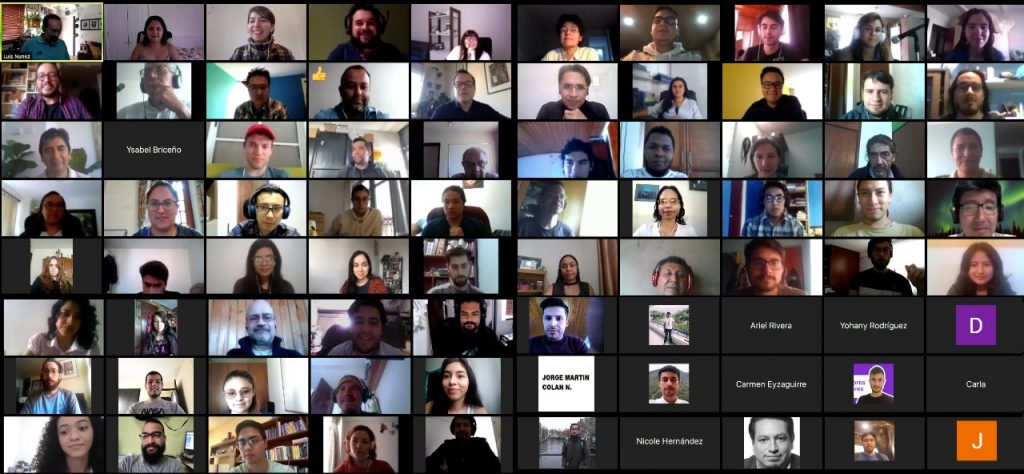
\includegraphics[scale=0.41]{imagenes/bienvenida-cohorte1-2.jpg}
\end{center}
%\end{columns}
\end{frame}

\begin{frame}[fragile]
\frametitle{LA-CoNGA hoy: 2021}
%\begin{columns}[c] % The "c" option specifies centered vertical alignment while the "t" option is used for top vertical alignment
%\column{.38\textwidth}
%aaa
%\column{.58\textwidth} % Right column and width
\begin{center}
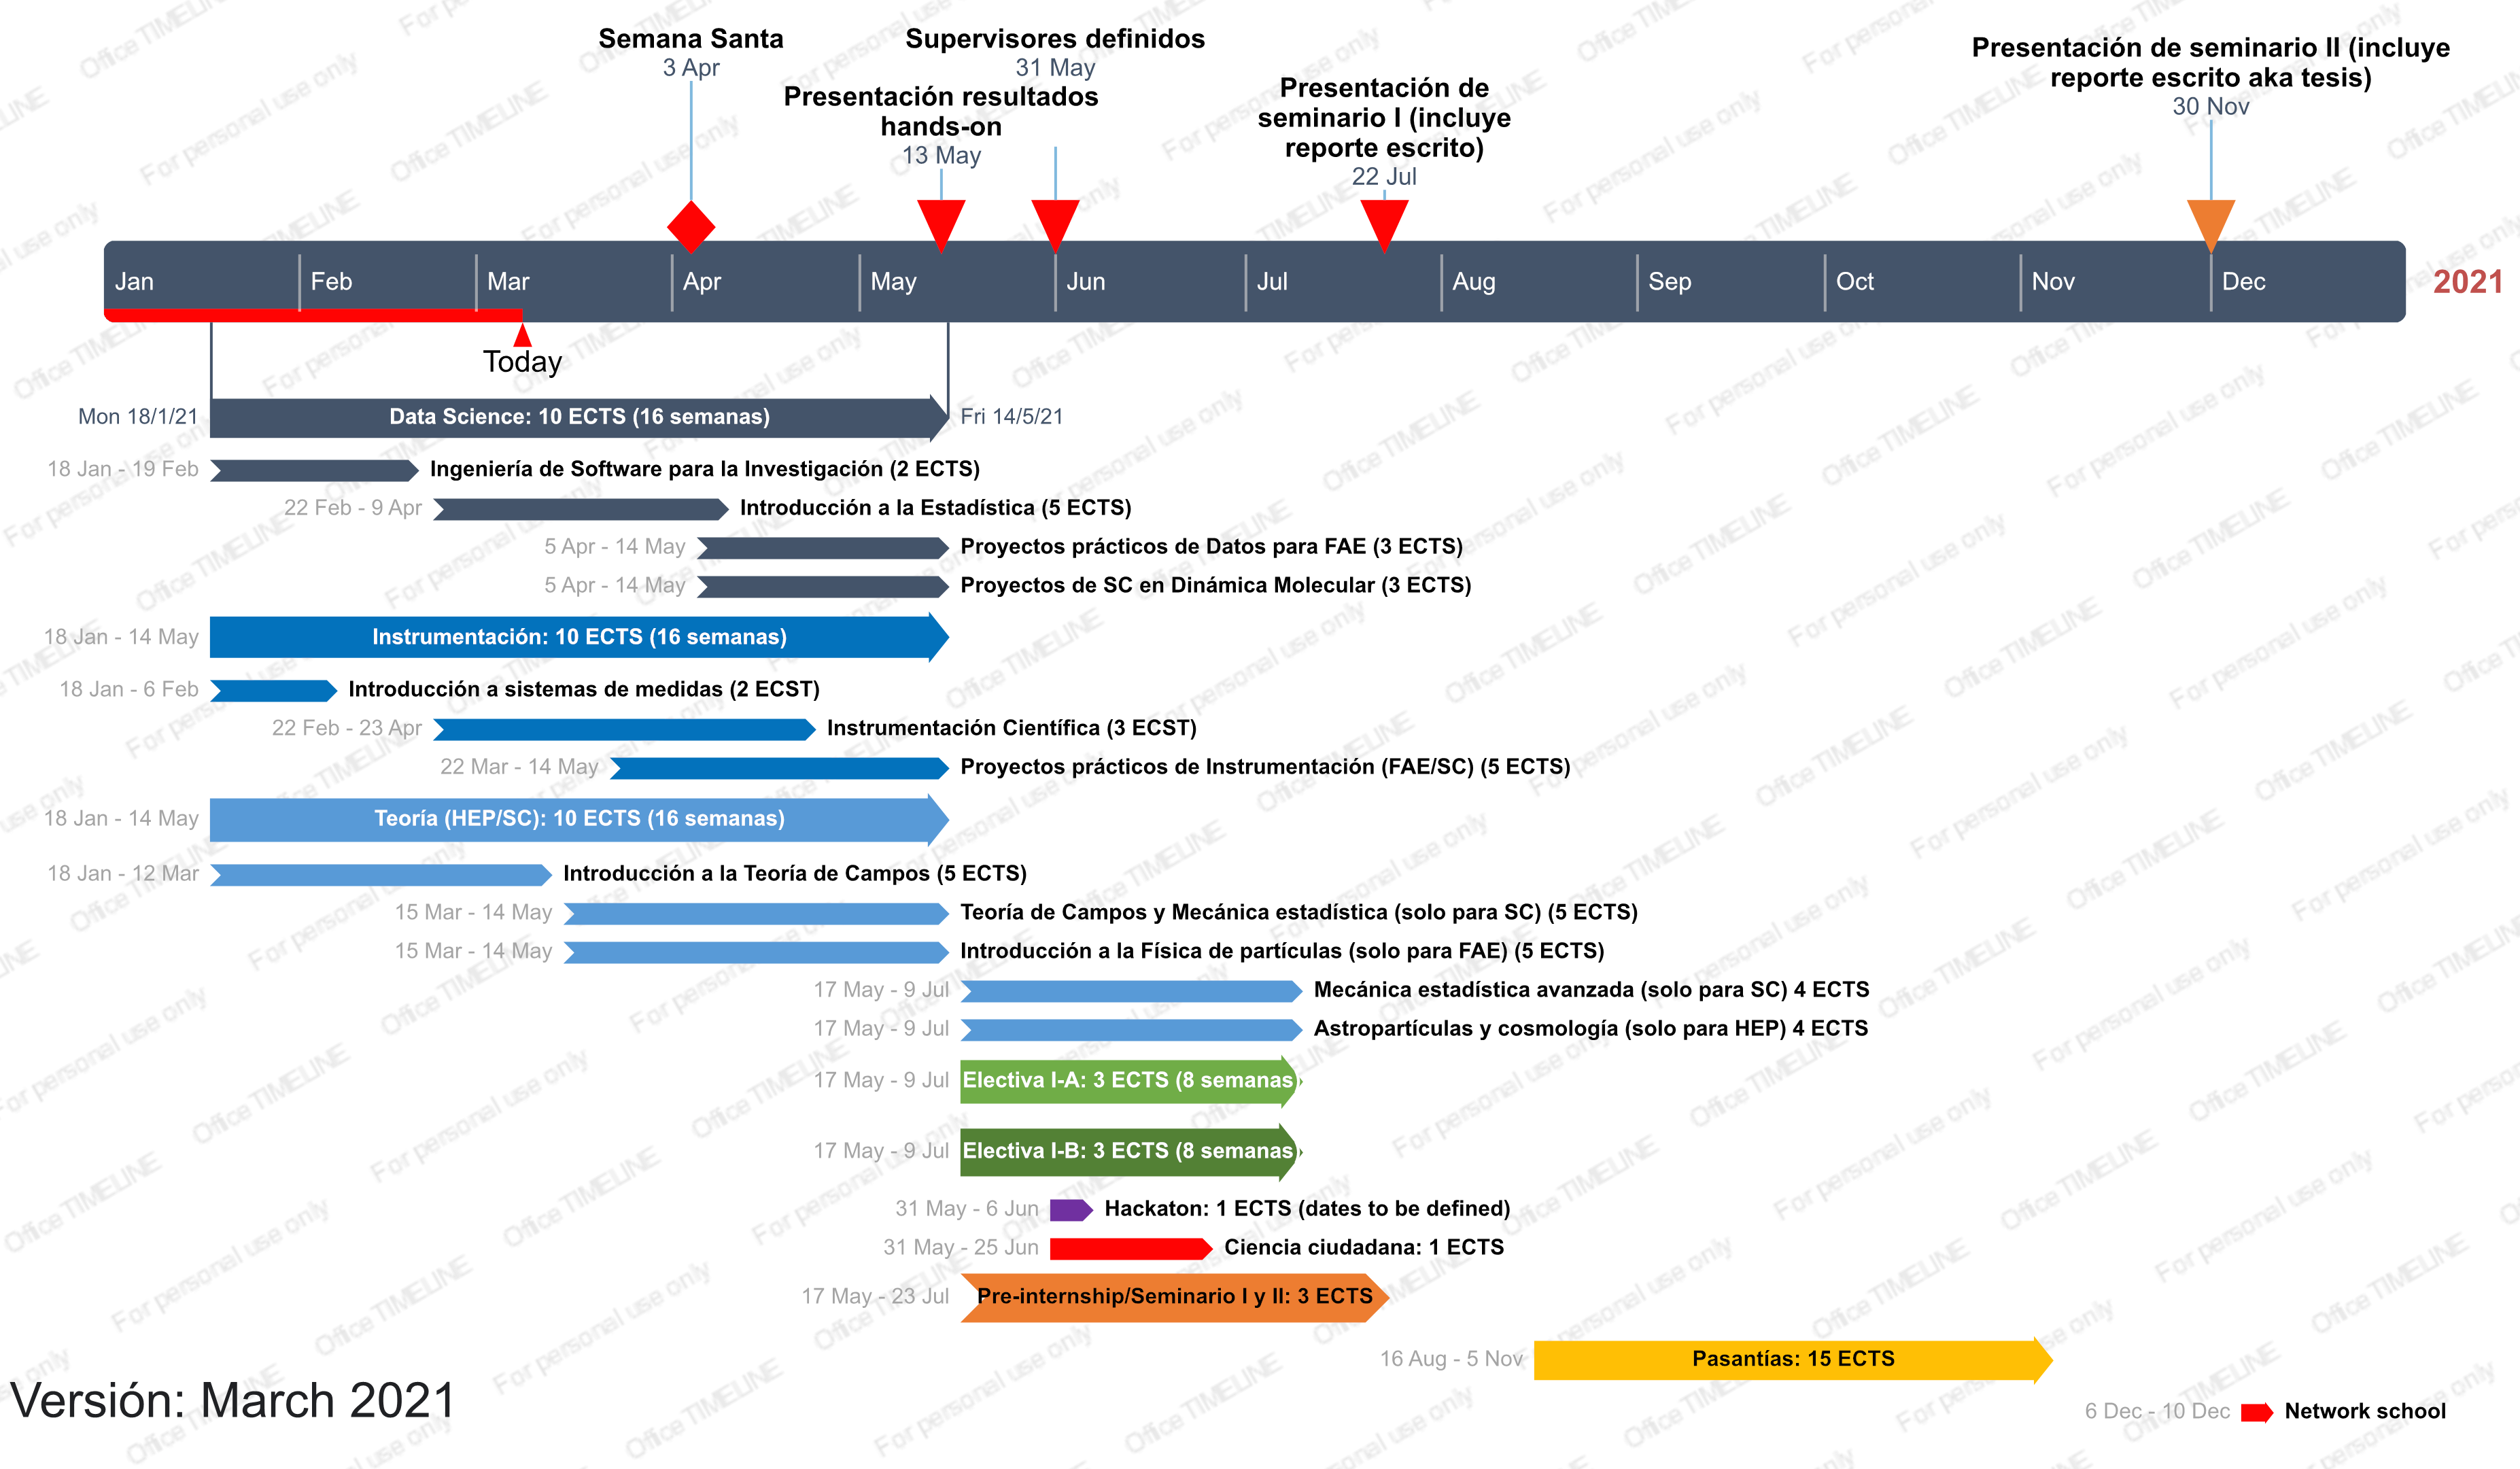
\includegraphics[scale=0.09]{imagenes/202103_GANTT_LA-CoNGA.png}
\end{center}
%\end{columns}
\end{frame}


\begin{frame}[fragile]
\frametitle{LA-CoNGA hoy: 2021}
%\begin{columns}[c] % The "c" option specifies centered vertical alignment while the "t" option is used for top vertical alignment
%\column{.38\textwidth}
%aaa
%\column{.58\textwidth} % Right column and width
\begin{itemize}
	\item Gestión académica
	\begin{itemize}
		\item Coordinación del equipo docente
		\item Acompañamiento a estudiantes: mentorías
		\item Accesibilidad
		\end{itemize}		
	\item Ajustes
	\begin{itemize}
		\item Currículo
		\item Plataforma
		\end{itemize}
	\item Plan de calidad
	\end{itemize}
%\end{columns}
\end{frame}

\begin{frame}[fragile]
\frametitle{LA-CoNGA mañana: 2022}

\begin{itemize}
	\item Segundo curso
	\item Plan de sostenibilidad, apropiación, integración, etc.
	\item Cierre del proyecto
	\end{itemize}
\end{frame}


%------------------------------------------------
%%%%%%%%%%%%%%%%%%
%%% Última lámina: fondo 9
%%%%%%%%%%%%%%%%%%
\usebackgroundtemplate{
\includegraphics[width=\paperwidth]{plantillas-laconga_9.jpg}}
\begin{frame}
%\Huge{\centerline{The End}}
\end{frame}

%----------------------------------------------------------------------------------------

\end{document}


\usebackgroundtemplate{
\includegraphics[width=\paperwidth]{plantillas-laconga_8.jpg}}
\begin{frame}
	\frametitle{Ecuaciones {\it serif}}
	\begin{equation}
		P^2=P^{\mu}P_{\mu}=m^2
	\end{equation}
	\begin{equation}
		x^2 + y^2 = r^2
	\end{equation}
\end{frame}

%\subsection{Subsection Example} % A subsection can be created just before a set of slides with a common theme to further break down your presentation into chunks

\usebackgroundtemplate{
\includegraphics[width=\paperwidth]{plantillas-laconga_8.jpg}}
\begin{frame}
\frametitle{Paragraphs of Text}
Sed iaculis dapibus gravida. Morbi sed tortor erat, nec interdum arcu. Sed id lorem lectus. Quisque viverra augue id sem ornare non aliquam nibh tristique. Aenean in ligula nisl. Nulla sed tellus ipsum. Donec vestibulum ligula non lorem vulputate fermentum accumsan neque mollis.\\~\\

Sed diam enim, sagittis nec condimentum sit amet, ullamcorper sit amet libero. Aliquam vel dui orci, a porta odio. Nullam id suscipit ipsum. Aenean lobortis commodo sem, ut commodo leo gravida vitae. Pellentesque vehicula ante iaculis arcu pretium rutrum eget sit amet purus. Integer ornare nulla quis neque ultrices lobortis. Vestibulum ultrices tincidunt libero, quis commodo erat ullamcorper id.
\end{frame}

%------------------------------------------------

\begin{frame}
\frametitle{Bullet Points}
\begin{itemize}
\item Lorem ipsum dolor sit amet, consectetur adipiscing elit
\item Aliquam blandit faucibus nisi, sit amet dapibus enim tempus eu
\item Nulla commodo, erat quis gravida posuere, elit lacus lobortis est, quis porttitor odio mauris at libero
\item Nam cursus est eget velit posuere pellentesque
\item Vestibulum faucibus velit a augue condimentum quis convallis nulla gravida
\end{itemize}
\end{frame}

%------------------------------------------------

\begin{frame}
\frametitle{Blocks of Highlighted Text}
\begin{block}{Block 1}
Lorem ipsum dolor sit amet, consectetur adipiscing elit. Integer lectus nisl, ultricies in feugiat rutrum, porttitor sit amet augue. Aliquam ut tortor mauris. Sed volutpat ante purus, quis accumsan dolor.
\end{block}

\begin{block}{Block 2}
Pellentesque sed tellus purus. Class aptent taciti sociosqu ad litora torquent per conubia nostra, per inceptos himenaeos. Vestibulum quis magna at risus dictum tempor eu vitae velit.
\end{block}

\begin{block}{Block 3}
Suspendisse tincidunt sagittis gravida. Curabitur condimentum, enim sed venenatis rutrum, ipsum neque consectetur orci, sed blandit justo nisi ac lacus.
\end{block}
\end{frame}

%------------------------------------------------

\begin{frame}
\frametitle{Multiple Columns}
\begin{columns}[c] % The "c" option specifies centered vertical alignment while the "t" option is used for top vertical alignment

\column{.45\textwidth} % Left column and width
\textbf{Heading}
\begin{enumerate}
\item Statement
\item Explanation
\item Example
\end{enumerate}

\column{.5\textwidth} % Right column and width
Lorem ipsum dolor sit amet, consectetur adipiscing elit. Integer lectus nisl, ultricies in feugiat rutrum, porttitor sit amet augue. Aliquam ut tortor mauris. Sed volutpat ante purus, quis accumsan dolor.

\end{columns}
\end{frame}



\begin{frame}
\frametitle{Table}
\begin{table}
\begin{tabular}{l l l}
\toprule
\textbf{Treatments} & \textbf{Response 1} & \textbf{Response 2}\\
\midrule
Treatment 1 & 0.0003262 & 0.562 \\
Treatment 2 & 0.0015681 & 0.910 \\
Treatment 3 & 0.0009271 & 0.296 \\
\bottomrule
\end{tabular}
\caption{Table caption}
\end{table}
\end{frame}

%------------------------------------------------

\begin{frame}
\frametitle{Theorem}
\begin{theorem}[Mass--energy equivalence]
$E = mc^2$
\end{theorem}
\end{frame}

%------------------------------------------------

\begin{frame}[fragile] % Need to use the fragile option when verbatim is used in the slide
\frametitle{Verbatim}
\begin{example}[Theorem Slide Code]
\begin{verbatim}
\begin{frame}
\frametitle{Theorem}
\begin{theorem}[Mass--energy equivalence]
$E = mc^2$
\end{theorem}
\end{frame}\end{verbatim}
\end{example}
\end{frame}

%------------------------------------------------

\begin{frame}
\frametitle{Figure}
Uncomment the code on this slide to include your own image from the same directory as the template .TeX file.
%\begin{figure}
%\includegraphics[width=0.8\linewidth]{test}
%\end{figure}
\end{frame}

%------------------------------------------------

\begin{frame}[fragile] % Need to use the fragile option when verbatim is used in the slide
\frametitle{Citation}
An example of the \verb|\cite| command to cite within the presentation:\\~

This statement requires citation \cite{p1}.
\end{frame}

%------------------------------------------------

\begin{frame}
\frametitle{References}
\footnotesize{
\begin{thebibliography}{99} % Beamer does not support BibTeX so references must be inserted manually as below
\bibitem[Smith, 2012]{p1} John Smith (2012)
\newblock Title of the publication
\newblock \emph{Journal Name} 12(3), 45 -- 678.
\end{thebibliography}
}
\end{frame}


